\section{Reading contract: what problem is being solved, and what evidence means}\label{reading-contract-what-problem-is-being-solved-and-what-evidence-means}

\subsection{The actual project problem}\label{the-actual-project-problem}

An input instance specifies a complete multi-output Boolean function

\[
F:\{0,1\}^{n}\to\{0,1\}^{m},\qquad 1\le n\le20,
\]

plus per-instance integer areas and propagation delays for \texttt{AND2}, \texttt{OR2} and \texttt{NOT}, a circuit-delay target, and optional program-runtime/RAM limits. The program must emit a legal topologically ordered netlist computing exactly the specified truth-table outputs. The target delay matters to quality, but \textbf{a functionally valid circuit above the target need not be a format/functional FAIL}. Conversely a timeout or failed resource check cannot be rescued by showing a low partial gate area. No numerical official grading formula was provided; consequently neither a home-made area--delay product (ADP) nor a sum of areas across diverse cases is called ``the official score.''

The legal network is a directed acyclic graph, not a collection of independent formulas. If \(L(G)\) is the set of gates reachable from the union of all primary outputs, area is

\[
A(G)=\sum_{v\in L(G)} a_{\operatorname{op}(v)},
\]

and critical-path delay is computed recursively, with primary inputs and the constant source arriving at zero:

\[
T(v)=d_{\operatorname{op}(v)}+\max_{u\in\operatorname{fanin}(v)}T(u),
\qquad D(G)=\max_{y\in\operatorname{outputs}}T(y).
\]

Write \(T_{\mathrm{synth}}(F,\pi)\) for the \emph{program's} elapsed synthesis time under policy \(\pi\), and \(M_{\mathrm{peak}}\) for measured resource consumption when available. These are different physical quantities from the circuit's gate delay. For every round, preserve four separate fields: \textbf{PASS/FAIL; target-met; charged Area; circuit Delay; synthesis Runtime} (and RAM where measured). Note that the report itself uses \textbf{five} status/metric fields because PASS and target-met are not synonyms.

\subsection{Four levels that must not be conflated}\label{four-levels-that-must-not-be-conflated}

\begin{enumerate}
\def\labelenumi{\arabic{enumi}.}
\tightlist
\item
  \textbf{Function:} the truth table defines \(F\); Boolean identities can prove exact equality.
\item
  \textbf{Intermediate representation:} Shannon DAG, ROBDD, complement reference or a small cut truth signature. A compact representation is not automatically an inexpensive netlist.
\item
  \textbf{Realized gate DAG:} exact AND2/OR2/NOT gates, fanout, liveness, weighted area and timing. A local syntax reduction need not remove a live gate.
\item
  \textbf{Search procedure:} how many mappings, cuts and roots the program visits before a wall-clock/resource limit. It is possible to improve level 3 while substantially worsening level 4.
\end{enumerate}

Stage 1's most useful lesson is the separation of these four objects. Stage 2 repeatedly encounters the \emph{same} distinction under tighter and more varied resource constraints.

\subsection{How the experimental records were audited}\label{how-the-experimental-records-were-audited}

The research bundle contains \texttt{01\_normalized\_data/runs.csv}, \texttt{case\_metrics.csv} and a content-addressed database \texttt{00\_inventory/payloads.sqlite}. For every one of the 1,706 run-index entries, the auditor retrieved the original report bytes using the stored report SHA-256, recomputed successful-case Area, Delay, number of PASS, number of target-met, and median success runtime, and reconciled them with the index. This included translating historical \texttt{True}/\texttt{False} target flags as well as newer \texttt{yes}/\texttt{no}. \textbf{All 1,706 indexed records matched} their original payloads; 602 unique report hashes were seen. This verifies extraction and arithmetic, \textbf{not} that every experiment was independently rerun or that duplicated copies count as new observations.

For the directly supplied late-round ZIP archives (R8.4--R10.1), the auditor read the named \texttt{experiment/official/} members for each bank, period and configuration directly and produced a second raw table and matched contrasts. Early R7--R8.3 reports were separately retrieved from the same content-addressed source store; their originating archive/member is stated in \texttt{runs.csv}. The R10.0 submitted \texttt{synth.cpp} and reproducibility snapshot have an identical SHA-256 beginning \texttt{8c863f1a...}; the Jincan R5.1 research source begins \texttt{cf90d0b1...}; the Zeyun submitted source begins \texttt{cd31f7d2...}. The two Stage 1 programs have different administrative and technical roles.

We classify observations as follows. \textbf{Direct matched evidence} uses identical bank, case, period and feedback experiment. \textbf{Archival development evidence} uses frozen historical outputs but may not control execution order or machine load. \textbf{Mechanism probes} hold one input DAG or a small constructed example fixed; they explain \emph{possibility} or a local intervention but not universal production behavior. \textbf{Code inspection} identifies the mechanism present in the frozen program; it does not prove which option fired on an uninstrumented historical run. Every number in a cross-version interpretation must be associated with one of these categories.

\subsection{The question-led roadmap --- not a changelog}\label{the-question-led-roadmap-not-a-changelog}

\begin{longtable}[]{@{}
  >{\raggedright\arraybackslash}p{(\columnwidth - 4\tabcolsep) * \real{0.3333}}
  >{\raggedright\arraybackslash}p{(\columnwidth - 4\tabcolsep) * \real{0.3333}}
  >{\raggedright\arraybackslash}p{(\columnwidth - 4\tabcolsep) * \real{0.3333}}@{}}
\toprule\noalign{}
\begin{minipage}[b]{\linewidth}\raggedright
Development problem
\end{minipage} & \begin{minipage}[b]{\linewidth}\raggedright
Experiment or intervention
\end{minipage} & \begin{minipage}[b]{\linewidth}\raggedright
Consequence for the next step
\end{minipage} \\
\midrule\noalign{}
\endhead
\bottomrule\noalign{}
\endlastfoot
Stage 1 establishes correctness but does not minimize a priced, timed shared graph & R1--R5.1: decomposition, portfolios, slack recovery, efficient typed DAG & Obtain a reliable, reasonably efficient full-circuit incumbent. \\
Local equivalences remain, but naive cut search is expensive & Stage 1 R6.0/R6.1 & Treat cut rewriting as a promising \textbf{research branch}, not a free default. \\
A faster kernel still misses a short-budget example & R7--R7.2 & Preserve a legal incumbent and admit optional search conservatively. \\
Pattern-only rewrites produce tiny, localized savings & R8 prototype & Search by small \textbf{Boolean function}, not only visible syntax. \\
More function choices can improve area at added circuit delay and synthesis time & R8.1--R8.2 & Separate feasibility, area-only policy, timing preference and search cost. \\
Wall limits make the set of visited nodes unstable & R8.3--R8.5 & Select/prioritize bounded \emph{work}, then study root allocation. \\
More time and more useful roots were confounded & R8.6 factorial study & The observed gains follow extra SOP roots, not nominal extra time. \\
Benchmark gains may not hold under fresh test families or tight budgets & R8.7--R9.0 & Freeze a safer runtime-first default plus an early structured bypass. \\
A new indexed library may discover more hits but save less area & R9.1 & Retain an ordinary repeat-SOP pass. \\
Deliverability needs a default policy rather than an environment switch & R10.0; R10.1 & Freeze R10.0 and reject unproductive reductions in its final budget. \\
\end{longtable}

This roadmap is a \emph{reading guide}. The evidence below is deliberately not represented as one monotone improvement curve.

\section{One recurring four-output example: why local rewriting must be tested globally}\label{one-recurring-four-output-example-why-local-rewriting-must-be-tested-globally}

The Stage 1 document used a three-input, two-output circuit to explain Shannon cofactors, shared timing and cut signatures. Stage 2 additionally needs a \textbf{four-output} example because shared outputs defeat naive algebraic cost arguments in an especially direct way. Let

\[
p=a\land b,\qquad q=a\land c,\qquad r=p\lor q,\qquad s=\neg r,
\]

and output all four signals \((p,q,r,s)\). Give AND2 area 2, OR2 area 3, NOT area 1, and corresponding delays 1, 2 and 1. The original DAG contains two AND gates, one OR gate and one NOT gate, so

\[
A(G)=2+2+3+1=8, \qquad D(G)=4.
\]

A symbolic optimizer notices \(r=(a\land b)\lor(a\land c)=a\land(b\lor c)\). As an isolated expression, factoring has fewer conjunctions. But because \(p\) and \(q\) are themselves primary outputs, both original AND gates remain live. We must now add the intermediate \(b\lor c\), an AND computing the newly factored \(r\), and keep the NOT for \(s\). Thus

\[
A(G')=2+2+3+2+1=10,\qquad D(G')=4.
\]

The factorization preserved \textbf{all} output truth functions but made the physical circuit \textbf{25\% more expensive}. This is not hypothetical: \texttt{06\_reproducibility/scripts/mechanism\_test.cpp} was independently compiled against the frozen R10.0 headers. It returned \texttt{factored=0\ area=8\ delay=4} and \texttt{factored=1\ area=10\ delay=4}, with identical root truth mask \texttt{168} in both cases; another 768 signature/mapping checks passed. It demonstrates the strict distinction between \textbf{Boolean correctness}, \textbf{local expression cost}, and \textbf{global output-reachable area}.

A second Stage 1 running example has \(f_1=(a\land b)\lor(\neg a\land c)\), \(f_2=f_1\lor b\). Replacing only the implementation of \(f_2\) with \(b\lor(\neg a\land c)\) leaves the shared \(f_1\) gate alive; its netlist area remains 11 but output delay drops from 7 to 5 under the reference gate costs. This is a \textbf{delay gain with zero area gain}. Together the two examples expose the central tension that later rounds must manage: equivalence proves \emph{legality of substitution}, not \emph{worth of substitution}.

For any two realized graphs with the same library costs,

\[
\Delta A=A(G')-A(G)
=\sum_{v\in L(G')\setminus L(G)}a_v
 -\sum_{v\in L(G)\setminus L(G')}a_v.
\]

This is a useful \textbf{exact accounting identity}, not a theorem that a particular candidate will have \(\Delta A<0\). It is why Stage 2 distinguishes estimates of \emph{private old cone reclaim} from final full-network acceptance.

\section{Transition: from Stage 1 evidence to Stage 2 constraints}
The preceding Stage 1 study already established a complete progression: exact Shannon/ROBDD construction, diversified mappings, slack-aware global recovery, typed DAG execution, and exploratory four-leaf cut rewriting. Its crucial unresolved problem was not whether cut rewriting \emph{could} save area---Rounds 6.0 and 6.1 measured real savings---but whether a function-level local search could be made valuable within the synthesizer's deadline and memory constraints. Stage 2 resumes precisely at this engineering question rather than starting the mathematical argument anew.

The separate actually submitted Stage 1 program (Z1) and Jincan's frozen R5.1 research program (J51) remain distinct. Z1 provides the assignment's formal submitted-stage comparator; J51 is the implementation-research lineage feeding into the R7--R10 development. Later matched evaluations of both programs are reported as distinct observations, not as a fabricated single lineage. The course specification, exact source snapshots, and raw results remain the authority for each claim.

\section{Round 7: when compiler optimization first exposed a feasibility cliff}\label{round-7-when-compiler-optimization-first-exposed-a-feasibility-cliff}

\subsection{The motivation was not simply to reduce area}\label{the-motivation-was-not-simply-to-reduce-area}

Entering Stage 2, the synthesizer must retain the existing exact representation and mapping portfolio but also survive short end-to-end runtime caps. Stage 1 had demonstrated that a cut search could be expensive; Stage 2 begins one level earlier: even finding the first valid candidate can consume too much time on particular tables. Round 7 starts from the frozen J51 source and experiments with the prime-implicant merge/greedy-cover computational kernels. Source switches \texttt{UFUG\_R7\_LEGACY\_MERGE} and \texttt{UFUG\_R7\_LEGACY\_COVER} permit restoration of the prior implementation for controlled comparison.

It is important to distinguish \textbf{algorithmic coverage} from \textbf{execution scheduling}. A faster kernel may reduce the cost of certain implicant operations but can also change which later portfolios reach a time gate; conversely the first candidate can still be too expensive on a short-limit example. There is no automatic theorem that a local kernel speedup guarantees end-to-end success.

\subsection{What the historical R7 controls actually showed}\label{what-the-historical-r7-controls-actually-showed}

In the R7 Audited Stage 2 comparison, the default modernized path had \textbf{24/25 PASS} (24/25 target met). Its \textbf{partial} area sum over 24 successes was 506,754 and successful-delay sum 1,065. The \texttt{legacy\_merge}, \texttt{legacy\_cover} and \texttt{legacy\_both} paths completed \textbf{25/25 PASS} and target-met cases, with complete area 508,535 and delay sum 1,101. The missing case was \textbf{Stage 2 / case\_016}, which had the short 100-ms cap. A 24-pass sum of 506,754 must not be called ``better area'' than 508,535 on 25 passes: an unreturned legal network has no comparable reported area.

Case 016 is a particularly useful falsification of the simplistic hypothesis ``large \(n\) is always the scheduling bottleneck.'' Its input dimension is modest, but the cap and specific search path are restrictive. The relevant principle is \textbf{time to produce an incumbent}, not input size alone; this log intentionally does not make the input-dimension distribution a separate research topic.

The audit's five variants and repeated case-specific profiling implicated the dispatch/search schedule, but archived aggregate CSVs are not a full event trace. We can say the default execution \textbf{failed under the limit} while legacy controls passed; we cannot infer which specific function call was always responsible without the matching trace.

\begin{tcolorbox}[colback=ResearchBlue!6!white,colframe=ResearchSlate!55!white,boxrule=0.65pt,arc=1mm,breakable]
\textbf{Decision after R7.} Prioritize \emph{obtaining a correct output before optional refinements}. Treat emergency guards as part of the algorithm's feasibility design. This shifts the central question from ``which kernel is fastest?'' to ``which candidate work should be admitted before the deadline?''
\end{tcolorbox}

\section{R7.1 and R7.2: a guard is necessary, but a blind guard throws away circuit quality}\label{r7.1-and-r7.2-a-guard-is-necessary-but-a-blind-guard-throws-away-circuit-quality}

\subsection{R7.1: the first attempt to protect the incumbent}\label{r7.1-the-first-attempt-to-protect-the-incumbent}

R7.1 applies a short-budget dispatch guard and tries to avoid late, expensive alternatives. In the frozen descendants, the guard's \emph{heuristic} admission line is visible: with a positive limit, \texttt{r71\_search\_cap} is 72\% of limits at most 250 ms, otherwise 75\%; later candidates are skipped when the elapsed launch time reaches this reserve. This is \textbf{not} hard preemption of C++ execution. Candidate constructors that ignore cancellation or cross a time check can still finish late.

R7.1's \texttt{r71\_guard} recovered the missing Stage 2 case and achieved \textbf{25/25 PASS, 25/25 target}, complete Stage 2 area \textbf{508,535}, delay sum \textbf{1,101} and one recorded median runtime \textbf{31.268 ms}. But \texttt{r71\_policy\_off} still had only 24/25. More revealingly, on Stage 1 / case\_020 the guarded path cost \textbf{777 area and 32 delay} whereas a corresponding legacy path gave \textbf{766 and 30}. That example is tiny in aggregate terms, yet conceptually decisive: a guard can preserve execution feasibility by prematurely suppressing useful cheap work. It is a \textbf{quality regression}, not a correctness failure.

\subsection{R7.2: conditional shortlisting rather than all-or-nothing search}\label{r7.2-conditional-shortlisting-rather-than-all-or-nothing-search}

R7.2's alternative is to keep the incumbent-first guard and selectively admit a \textbf{bounded shortlist} where time remains. The frozen descendant exposes \texttt{UFUG\_R72\_POLICY} for \texttt{guard}, \texttt{shortlist} and \texttt{nocancel} behavior, with a stricter admission test and checkpoint/cancellation diagnostics. The intended logical distinction is: do not restart a risky full search, but do not assume that every optional candidate is equally expensive or equally useless.

In the two-bank R7.2 feedback (two periods), Stage 2 \texttt{r72\_guard}, \texttt{r72\_nocancel}, \texttt{r72\_shortlist} and the comparator achieved 25 PASS and target met, with area \textbf{508,535} and delay \textbf{1,101} under the successful reported runs. The Stage 2 medians in one run were approximately 31.033, 29.846 and 30.489 ms for the three R7.2 policies, compared with 29.985 ms for \texttt{r71\_guard}; none should be ranked as universally faster on this small difference. The \textbf{Stage 1 / case\_020} correction, by contrast, separates policies more clearly: \texttt{shortlist} and \texttt{nocancel} restore the baseline network quality while \texttt{guard} retains an 11-area regression.

\subsection{The decision that survived}\label{the-decision-that-survived}

The final scheduling rule learned from R7--7.2 is not ``always run less'' and not ``always run the fastest branch.'' It is a two-layer feasibility strategy: (i) establish and preserve a legal incumbent; (ii) spend remaining time on the most plausibly useful extra work, with a conservative admission guard. Later R9 and R10 keep that principle when adding expensive cut passes, so the R7 family is a genuine \textbf{architectural prerequisite}, not a disposable preface.

\section{Round 8 prototype: why algebraic patterns and iterations were a necessary but insufficient probe}\label{round-8-prototype-why-algebraic-patterns-and-iterations-were-a-necessary-but-insufficient-probe}

\subsection{The research question and its origin in R6}\label{the-research-question-and-its-origin-in-r6}

Having restored an incumbent-first runtime discipline, the next task was to find lower-area implementations of a circuit that already passed. One could simply revisit the original truth table with a new variable order, but that does not directly change a \emph{particular expensive gate pattern in the emitted DAG}. Stage 1 R6 had shown that local resynthesis was possible, although expensive. Round 8 therefore starts with cheaper, narrower structural interventions: factoring visible shapes, reusing identical algebraic substructures and running a small number of repeat cleanup passes.

The principle is elementary but nontrivial under sharing: Boolean operators are associative, distributive and absorb certain repeated terms, yet a substitution may change a network's fanout, liveness and critical path. The prototype deliberately tests \texttt{off}, \texttt{factor}, \texttt{reuse}, \texttt{strict}, \texttt{all} and \texttt{iterate} instead of assuming every rewrite can safely be composed. The corresponding code is retained in \texttt{r8\_structural.hpp} and called by the frozen descendant through the optional \texttt{UFUG\_R8\_POLICY} branch. Later production runs default \textbf{away} from this research branch, because the more general cut search supersedes it.

\subsection{Interpreting the experiment at the proper unit}\label{interpreting-the-experiment-at-the-proper-unit}

On the 25 Stage 1 published cases, the R8 prototype and R7.2 remained at 529,014 area and all 25 met target, across both recorded periods. On Stage 2, R7.2 area was 508,535; \texttt{factor} and \texttt{strict} also gave 508,535; \texttt{reuse} and \texttt{all} gave 508,523; and \texttt{iterate} gave \textbf{508,480}. The gain of 55 comes entirely from a localized opportunity on Stage 2 / case\_021. In an offline five-pass trace of that same example, successive extra area savings were 12, 35, 4, 4 and 0. Its delay moved from 69 to 70 while remaining feasible. The complete Stage 2 delay sum consequently moved from 1,101 to 1,102. Both public periods reproduced these area totals.

The fourth and fifth passes are a warning about convergence language. A zero \emph{next-pass} gain is evidence of a local fixed point \textbf{under the current rule, order and remaining graph}; it is not proof of minimum-area realization. And the gains cannot be divided into independent treatment effects because each pass changes the input graph of the next one. Formally, if \(P\) denotes one cleanup pass, the observed sequence concerns

\[
G_0,\quad G_1=P(G_0),\quad G_2=P(G_1),\ldots,
\]

not repeatedly applying \(P\) to the \emph{same} fixed \(G_0\). Thus \(A(G_0)-A(G_2)\) contains a path-dependent interaction, not necessarily the sum of two isolated gains.

\subsection{What R8 resolved and what it did not}\label{what-r8-resolved-and-what-it-did-not}

The prototype establishes three narrow facts: a completed legal incumbent can still contain profitable local structure; structural cleanup can expose further opportunities for subsequent passes; and a modest area gain can coexist with a small delay increase while preserving the target. It does \textbf{not} establish that factoring is broadly effective or that iteration is worth deploying on all functions. The research question becomes sharper: can a rewrite be driven by the \textbf{actual Boolean function of a bounded cone}, independent of the syntactic pattern in which it happens to appear? That is the transition to R8.1.

\section{Round 8.1: the central change of object --- from syntax patterns to 4-leaf truth functions}\label{round-8.1-the-central-change-of-object-from-syntax-patterns-to-4-leaf-truth-functions}

\subsection{A cut is a function boundary, not a substring of the netlist}\label{a-cut-is-a-function-boundary-not-a-substring-of-the-netlist}

For a root gate \(v\), a cut \(C=\{\ell_1,\ldots,\ell_k\}\) is a set of upstream frontier signals that intercepts every backward path from \(v\) to a primary source. A \emph{feasible} cut has \(k\le4\). After replacing the upstream cone behind that frontier by formal variables \(z_1,\ldots,z_k\), the root is a Boolean function \(h_{v,C}:\{0,1\}^k\rightarrow\{0,1\}\). Its truth mask is

\[
M(v,C)=\sum_{s=0}^{2^k-1} h_{v,C}(s)2^s,
\qquad 0\le M<2^{2^k}\le2^{16}.
\]

The maximum 16-bit mask is computationally cheap to enumerate. The mask is a \emph{semantic bridge}: it forgets the particular sequence of AND, OR and NOT gates in the original cone while preserving its function on the cut inputs. This is a qualitatively different search space from identifying only a literal distributive or absorption pattern.

\textbf{Why exact equality is sufficient even with correlated leaves.} In a real circuit the leaf signals \((\ell_1(x),\ldots,\ell_k(x))\) need not realize all \(2^k\) Boolean assignments. Nevertheless, if a candidate \(\tilde h\) matches \(h_{v,C}\) on \textbf{all} formal assignments, then for every primary input vector \(x\),

\[
\tilde h\bigl(\ell_1(x),\ldots,\ell_k(x)\bigr)
=h_{v,C}\bigl(\ell_1(x),\ldots,\ell_k(x)\bigr).
\]

This proves local functional substitution unconditionally, without making any stochastic-independence assumption about the leaf signals. Equality on all formal assignments is often stronger than necessary when leaves are correlated, but is an easily checked sufficient test. It says \emph{nothing by itself} about new graph cycles, other output uses, exact area or arrival times; those must be checked separately.

\subsection{The actual candidate families and mapping costs}\label{the-actual-candidate-families-and-mapping-costs}

The R8.1 family expands each small cut by several choices. One is Shannon decomposition along an ordering \(\sigma\):

\[
h(z_1,\ldots,z_k)
=\bigl(\neg z_{\sigma(1)}\land h_0\bigr)
 \lor\bigl(z_{\sigma(1)}\land h_1\bigr),
\]

recursively reducing cofactors until they are constants. Other choices enumerate exact implicants of the positive truth mask, build an SOP, enumerate the complement mask and invert its SOP (a POS-like realization), and vary the greedy-cover policy. Every XOR-like or multiplexer-like intermediary must eventually be lowered to permitted AND2/OR2/NOT gates. These alternatives are \emph{exact Boolean implementations}, not approximate learned surrogates.

In the frozen descendant \texttt{r84\_cut.hpp}, \texttt{truth()} (lines approximately 132--150) recursively computes the bit mask with \texttt{AND}/\texttt{OR}/mask complement and throws if a path bypasses the cut frontier; \texttt{Env::sop()} (approximately 69--105) enumerates prime cubes for no more than four leaves; \texttt{Env::build\_shannon()} (approximately 106--129) constructs a mapped decomposition; and \texttt{private\_reclaim()} (approximately 164--177) accounts conservatively for the old cone by refusing to count multi-fanout predecessors as removable. The source lineage confirms that these are concrete implementations of the R8 family, although a frozen R10 header must not be mistaken for a byte-identical R8.1 executable.

Suppose \(\widehat A_{\rm new}\) is the emitted cost of a candidate cone relative to the same mapped frontier, and \(\widehat A_{\rm reclaim}\) is the conservative cost of private old gates expected to become dead. The local screening proxy is

\[
\widehat{\Delta A}=\widehat A_{\rm new}-\widehat A_{\rm reclaim}.
\]

A favorable local proxy merely justifies considering the candidate. Hash-consing may reuse gates that appear outside the cone; original gates may remain live because of other fanouts; and in-place rewriting can alter reachability. The final acceptance test is on a \textbf{finished live DAG}, not on this estimate. That distinction was already foreshadowed by Stage 1's algebra/fanout example and is now encoded in the synthesizer.

\subsection{Required time is a feasibility screen, not a score}\label{required-time-is-a-feasibility-screen-not-a-score}

Let \(R(y)\) initially equal the target delay for each output. On an unchanged DAG, backward propagation gives

\[
R(u)=\min_{v:\,u\in\mathrm{fanin}(v)}\bigl(R(v)-d_{\operatorname{op}(v)}\bigr),
\]

also taking the primary-output target if \(u\) itself is an output. A candidate root with new arrival \(T'(v)\le R(v)\) can be feasible under a fixed external boundary even if its arrival increases. For the Stage 1 running example, a signal that serves both as output and downstream fanin can have a tighter required time than its own output deadline. The old \(R\) values are \textbf{not safe to reuse after arbitrary fanout restructuring}; the final full-DAG metric is authoritative.

A formal sufficient condition holds if the rest of the DAG retains its dependencies and gate delays and each new boundary root meets its original required arrival. Topological induction then shows that every unchanged successor meets its old required arrival and all output delays remain within target. But this lemma is not a universal proof for freely restructured graphs. Stage 2's implementation combines local screening with a final completed-network feasibility check for exactly this reason.

\subsection{What R8.1 actually found: area and delay can pull in different directions}\label{what-r8.1-actually-found-area-and-delay-can-pull-in-different-directions}

The first archived Stage 2 experimental period provides the clearest contrast. All variants below have 25 PASS and 25 target-met cases:

\begin{longtable}[]{@{}
  >{\raggedright\arraybackslash}p{(\columnwidth - 6\tabcolsep) * \real{0.2500}}
  >{\raggedleft\arraybackslash}p{(\columnwidth - 6\tabcolsep) * \real{0.2500}}
  >{\raggedleft\arraybackslash}p{(\columnwidth - 6\tabcolsep) * \real{0.2500}}
  >{\raggedleft\arraybackslash}p{(\columnwidth - 6\tabcolsep) * \real{0.2500}}@{}}
\toprule\noalign{}
\begin{minipage}[b]{\linewidth}\raggedright
R8.1 policy, Stage 2 period 1
\end{minipage} & \begin{minipage}[b]{\linewidth}\raggedleft
Charged area
\end{minipage} & \begin{minipage}[b]{\linewidth}\raggedleft
Sum of output delays
\end{minipage} & \begin{minipage}[b]{\linewidth}\raggedleft
Median synthesizer runtime (ms)
\end{minipage} \\
\midrule\noalign{}
\endhead
\bottomrule\noalign{}
\endlastfoot
Prior R7.2 reference & 508,535 & 1,101 & approximately 32--35 in its own feedback \\
\texttt{r81\_strict} & 508,326 & 1,101 & 193.074 \\
\texttt{r81\_sop} & 498,949 & 1,161 & 95.509 \\
\texttt{r81\_shannon} & 498,568 & 1,158 & 95.287 \\
\texttt{r81\_reverse} & \textbf{497,509} & \textbf{1,158} & 189.880 \\
\end{longtable}

The R7.2 runtime is listed only for context from \textbf{a separate feedback batch}, so its subtraction from the R8.1 medians is \emph{not} a matched speedup/slowdown measurement. Inside the R8.1 batch, the policies themselves are comparable. The \texttt{reverse} policy saves 11,026 charged area units relative to the archived R7.2 area reference, at an increase of 57 in aggregate circuit delay. \texttt{strict} saves only 209 yet does not increase the aggregate delay. The former is not ``better in every metric''; the latter is not ``useless.''

On Stage 2 / case\_005, \texttt{r81\_reverse} yields area \textbf{106,770}, \texttt{r81\_strict} \textbf{112,221}; on case\_003 the corresponding areas are \textbf{15,207} and \textbf{19,494}. These are \emph{actual per-case} manifestations of how candidate admission matters. Neither comparison establishes the hidden evaluator's score, and sum of delays is descriptive rather than a universal quality utility.

\subsection{Decision after R8.1}\label{decision-after-r8.1}

R8.1 validates the central method hypothesis: bounded Boolean-function rewriting exposes substantially more area opportunities than sparse syntax patterns. But a policy that ``takes every legal cheaper cone'' can consume significant synthesis time and relax non-regression of individual delays as long as the target is still met. The next question is therefore not ``does cut rewriting work?'' It is \textbf{which search and acceptance objective should be used, and how much of the search should be done per instance?} R8.2 turns those choices into controlled alternatives.

\section{Round 8.2 and 8.2.1: choosing a point in a multi-dimensional engineering problem}\label{round-8.2-and-8.2.1-choosing-a-point-in-a-multi-dimensional-engineering-problem}

\subsection{R8.2: area-first, slack-first and ADP-style rankings are different policies}\label{r8.2-area-first-slack-first-and-adp-style-rankings-are-different-policies}

The combinational function must remain exact in every mode; what changes is the ordering and acceptance of legal candidates. An area-oriented policy prioritizes \(A(G)\) subject to timing feasibility. A more conservative policy can prefer preserving or reducing \(D(G)\), even after the target is met. An internal area--delay-product proxy, \(A(G)D(G)\), trades both by multiplying them. It is mathematically a well-defined search heuristic, but it is \textbf{not} the published course-score function and should never be presented as such.

For small perturbations,

\[
\frac{\Delta(AD)}{AD}\approx\frac{\Delta A}{A}+\frac{\Delta D}{D}.
\]

This explains why a candidate offering a small area saving can be rejected by an ADP objective when it increases delay enough. A weighted lexicographic or target-feasible objective can make the opposite decision. The hypotheses are genuinely different; they cannot be evaluated merely by renaming the same area total.

Round 8.2 added fast and dual-branch variants, slack-oriented and ADP choices, and different root sampling/traversal rules. In its own \textbf{Stage 2 period-one} records, all 25 cases passed and met target, but outcomes diverged:

\begin{longtable}[]{@{}lrrr@{}}
\toprule\noalign{}
R8.2 Stage 2 policy & Area & Delay sum & Median runtime (ms) \\
\midrule\noalign{}
\endhead
\bottomrule\noalign{}
\endlastfoot
\texttt{r82\_dual\_area} & \textbf{501,547} & 1,156 & 163.231 \\
\texttt{r82\_fast\_area} & 503,313 & 1,137 & 163.812 \\
\texttt{r82\_fast\_slack} & 506,296 & 1,109 & 156.450 \\
\texttt{r82\_fast\_adp} & 508,380 & \textbf{1,101} & 154.480 \\
\end{longtable}

The dual-area policy achieves lower area than fast-area on this bank; it does so at a greater total circuit delay. The ADP variant retains the original delay sum but gains comparatively little area. Thus \emph{target feasibility} and \emph{delay non-regression} induce different feasible choices. The precise optimal choice cannot be deduced from area or ADP alone without the official score and resource distribution.

The independent repeated period reports another area for some dual searches, consistent with wall-clock-dependent candidate trajectories. It is inappropriate to call two totals recorded on different invocations a perfectly stable deterministic cost function when a time gate can change which roots are reached.

\begin{tcolorbox}[colback=ResearchBlue!6!white,colframe=ResearchSlate!55!white,boxrule=0.65pt,arc=1mm,breakable]
\textbf{Decision after R8.2:} preserve multiple frozen comparators, rather than prematurely declaring a universal area/delay/runtime winner. Add explicit resource handling and then separate variability in the root-search process from the underlying Boolean opportunities.
\end{tcolorbox}

\subsection{R8.2.1: program resource limits are not the same as circuit properties}\label{r8.2.1-program-resource-limits-are-not-the-same-as-circuit-properties}

The input format can specify a ninth-line RAM limit. The algorithm therefore must distinguish (i) a correctness-preserving compact alternative, (ii) deciding whether a BDD or truth-table representation is \emph{admissible} under a conservative memory estimate, and (iii) the evaluator's external memory supervision. The frozen \texttt{r821\_resource.hpp} and R10.0 entry code parse both optional positive limits; the latter may attempt a compact exact solver or decline an estimated inadmissible BDD route instead of blindly using memory.

The R8.2.1 probe deliberately used a tiny exact-wire C solver as a control. One archived low-RAM experiment returned evaluator \texttt{MEMORY\_LIMIT} at \textbf{9,000 KiB}, while a separate direct process monitor reported only \textbf{1,344 KiB} high-water resident memory for the tiny program. The two observations use different measurement layers. They expose a \textbf{measurement/interface discrepancy worth investigating}; they do not prove that the evaluator has a bug, reveal its monitoring internals, or establish a universal memory threshold. There are additional patched and clean evaluator probes, which must be identified by their exact run directory when cited.

The code can formally reject an obviously too-large representation \emph{relative to its estimate}, but it cannot guarantee the evaluator will accept every low-memory execution. Likewise passing a small probe does not prove correctness for all 20-input instances. The lasting contribution of R8.2.1 is clearer resource accounting and honest limits on what a memory measurement certifies, not a new Boolean minimization method. Keep this branch proportionate in the Stage 2 paper; preserve the full detail here because it explains why ``PASS'' includes more than Boolean equivalence.

\section{Round 8.3: make the amount of search work explicit}\label{round-8.3-make-the-amount-of-search-work-explicit}

\subsection{The problem hidden inside an elapsed-time cutoff}\label{the-problem-hidden-inside-an-elapsed-time-cutoff}

Cut rewriting is an \emph{ordered search}. Let \(r_1,\ldots,r_N\) be eligible roots and let \(C(r_i,G)\) denote the work required to examine the cuts of root \(r_i\) in the current mapped network. Under a wall-time limit \(B\), the number of roots visited is not fixed. It depends on data structures, CPU load and the changing shape of \(G\):

\[
K(B,G,\mathrm{machine})=
\max\biggl\{k:\sum_{i=1}^{k}C(r_i,G)\lesssim B\biggr\}.
\]

The expression is schematic, not a claim that runtime is a literal sum of independent root costs: caching, graph growth and periodic clock checks couple the terms. Its purpose is to show why the \emph{same} wall allowance need not produce the same visited search set. Because accepted rewrites alter the subsequent graph, missing or gaining a root can produce different final area, even with the same source and input.

Round 8.3 introduces a deterministic \textbf{root-work quota} alongside an emergency wall guard. The former controls an algorithmic quantity (number of completed selected roots), while the latter guards end-to-end runtime. This does not produce deterministic total running time, because one root can contain many cuts and candidates; it does make one dimension of the search more reproducible. In the frozen \texttt{r84cut::rewrite}, \texttt{visited\_roots} is checked against \texttt{work\_roots} at a root boundary; a clock check is performed periodically. Any remaining unprocessed original nodes are copied to finish a legal graph. This last operation is essential: an optimization timeout is allowed to truncate extra research but not to leave an incomplete netlist.

\subsection{\texorpdfstring{9.2 A quota controls effort but also changes \emph{which} root wins}{9.2 A quota controls effort but also changes which root wins}}\label{a-quota-controls-effort-but-also-changes-which-root-wins}

The R8.3 Stage 2 period-one feedback compares a prior \texttt{r821\_dual\_area} with \texttt{r83\_stable\_dual}, \texttt{r83\_dense\_dual} and \texttt{r83\_fast\_area}. All four complete 25/25 cases and their delay targets, but differ materially:

\begin{longtable}[]{@{}lrrr@{}}
\toprule\noalign{}
R8.3 comparison & Area & Delay sum & Median runtime (ms) \\
\midrule\noalign{}
\endhead
\bottomrule\noalign{}
\endlastfoot
\texttt{r821\_dual\_area} & 493,922 & 1,169 & 131.044 \\
\texttt{r83\_dense\_dual} & 497,885 & 1,169 & 126.208 \\
\texttt{r83\_stable\_dual} & 500,072 & 1,169 & 87.518 \\
\texttt{r83\_fast\_area} & 502,717 & 1,137 & 58.628 \\
\end{longtable}

These within-batch differences are descriptive tradeoffs, not clean estimates of one isolated code change. Stable work reduces some wall variability but can exclude useful roots that an earlier, more opportunistic schedule happened to visit. For example, on Stage 2 / case\_003 the selected areas move from 15,318 (\texttt{r821\_dual\_area}) to 17,283 (\texttt{stable\_dual}), whereas case\_005 moves from 102,928 to 106,771. The numerical pattern does not prove that one root-ranking heuristic is universally optimal; it motivates examining \textbf{what was selected by the quota}.

\begin{tcolorbox}[colback=ResearchBlue!6!white,colframe=ResearchSlate!55!white,boxrule=0.65pt,arc=1mm,breakable]
\textbf{Decision after R8.3:} root-count stability alone is insufficient. A bounded search should spend its fixed work quota on promising roots, where ``promising'' must be defined by a proxy tied to removable live area and timing slack. That leads to R8.4.
\end{tcolorbox}

\section{Round 8.4: priority ranking, topological traversal and the Top-Q distinction}\label{round-8.4-priority-ranking-topological-traversal-and-the-top-q-distinction}

\subsection{Why ``rank 1,500, then visit the first 900'' is not ``visit the best 900''}\label{why-rank-1500-then-visit-the-first-900-is-not-visit-the-best-900}

A DAG can be rewritten safely in a topological pass because mapped predecessors are ready before their consumers. But ranking roots by potential benefit and \emph{visiting them} are two separate operations. One historical scheme retained a high-ranked pool, then visited up to a quota in ascending topological order. The selected set can differ radically from the highest-scored \(Q\) roots even though both schemes report the same nominal quota.

Let \(s(v)\) be a root priority proxy, and \(P_K\) be the best \(K\) roots by that proxy. Then the historical policy selects the first \(Q\) root IDs in \(\mathrm{sort}_{\mathrm{topological}}(P_K)\), while a \textbf{Top-Q policy} first chooses \(P_Q\) and \emph{then} traverses that selected set topologically. They differ whenever relative topological position and rank disagree:

\[
\mathrm{first}_{Q}\bigl(\mathrm{toposort}(P_K)\bigr)
\ne P_Q,\qquad Q<K.
\]

The distinction matters because an early low-ID root may be less promising but can be reached before a higher-value later root. Conversely, the chosen root set affects structural opportunities created for downstream replacements. A ranking is only a heuristic; the exact payoff is measured after completing the network.

The frozen \texttt{r84\_cut.hpp} defines a score whose principal terms are gate area and one-hop private predecessors:

\[
s(v)=16a(v)+8\sum_{u\in\mathrm{fanin}(v)\atop u\text{ internal},\ \mathrm{use}(u)=1}a(u)
+\min\{8,\max(0,R(v)-T(v))\}.
\]

This is a \textbf{selection surrogate}, not the true benefit of rewriting \(v\). It approximates reclaimable private gates plus slack; it does not forecast which Boolean candidate will materialize. The root population is first ranked by this proxy, Top-Q membership is fixed where selected, and the actual rewrite remains topological. R8.4 also compares mixed quotas and pilot→focus allocation for the two branch families.

\subsection{The R8.4 controlled outcomes resist an easy ranking story}\label{the-r8.4-controlled-outcomes-resist-an-easy-ranking-story}

In the first R8.4 Stage 2 period, with 25 PASS/target cases throughout:

\begin{longtable}[]{@{}lrrr@{}}
\toprule\noalign{}
Strategy & Area & Delay sum & Median runtime (ms) \\
\midrule\noalign{}
\endhead
\bottomrule\noalign{}
\endlastfoot
\texttt{r84\_topology\_dual} & \textbf{501,063} & 1,169 & 206.012 \\
\texttt{r84\_topq\_dual} & 501,124 & 1,170 & 182.445 \\
\texttt{r84\_topq\_dense} & 500,027 & 1,170 & 191.486 \\
\texttt{r84\_adaptive\_dual} & 502,266 & 1,172 & 213.674 \\
\end{longtable}

\texttt{topq\_dense} improves area relative to both \texttt{topology\_dual} and \texttt{topq\_dual} in that first invocation, but the second period changes the ranking of some alternatives. Even the simpler \texttt{topology\_dual}→\texttt{topq\_dual} comparison illustrates why a theoretically more ``faithful'' priority ranking does not automatically improve the finished circuit: area moves from 501,063 to 501,124, and delay sum from 1,169 to 1,170. On case\_003, by contrast, Top-Q lowers area from 17,283 to 16,213; on case\_005, it increases area from 107,754 to 109,084. The mixed population explains the small aggregate reversal.

This is \textbf{not} evidence against ranking per se. It is evidence that the priority formula, downstream sharing, order of accepted transformations and finite root quota interact. The right next experiment is to control the scheduling of the \textbf{two candidate-generation branches}, not to assume a single root-score formula solves every case.

\begin{tcolorbox}[colback=ResearchBlue!6!white,colframe=ResearchSlate!55!white,boxrule=0.65pt,arc=1mm,breakable]
\textbf{Decision after R8.4:} retain Top-Q and dense variants as controlled choices, but study whether SOP and Shannon should be ordered or budgeted differently. R8.5 takes that step.
\end{tcolorbox}

\section{Round 8.5: branch-order search and the confounding of additional work with additional time}\label{round-8.5-branch-order-search-and-the-confounding-of-additional-work-with-additional-time}

\subsection{Two passes may be compositional, but comparison must hold the input fixed}\label{two-passes-may-be-compositional-but-comparison-must-hold-the-input-fixed}

The cut optimizer can generate SOP-like and Shannon-like candidates. Two possible full-pass orders are \(H\rightarrow P\) (Shannon then SOP) and \(P\rightarrow H\) (SOP then Shannon). If the second pass operates on the output of the first, the maps need not commute:

\[
P(H(G))\ne H(P(G)).
\]

The equality of the \emph{Boolean outputs} does not make their gate DAGs identical. The first pass changes cut frontiers, hashing opportunities, arrival times and which private gates survive. A second pass may discover something newly visible, or lose a formerly available structural match. There is no general theorem that SOP-first always wins.

In R8.5's first Stage 2 run, \texttt{r85\_shannon\_first}, \texttt{r85\_sop\_first} and \texttt{r84\_topq\_dual} all yielded \textbf{area 497,785}, delay \textbf{1,170}, with medians 92.541, 90.418 and 93.720 ms respectively. The tie is \textbf{conditional on these runs}: it does not prove the order commutes on all graphs. The \texttt{r85\_budget\_reclaim} configuration yielded the stronger \textbf{494,999} at the same delay, but it modified not only the traversal order: unused time could be reallocated to the next branch, changing its potential work as well.

\subsection{Why the R8.5 result cannot identify its own mechanism}\label{why-the-r8.5-result-cannot-identify-its-own-mechanism}

If policy A changes both the SOP root quota and time allowance, an improvement in output area can result from either factor or their interaction. Let \(A_{qr}\) denote area with root-quota treatment \(q\in\{0,1\}\) and time-reclaim treatment \(r\in\{0,1\}\). Observing just \(A_{00}\) and \(A_{11}\) identifies only the \textbf{joint intervention}, not the partial effects \(A_{10}-A_{00}\) and \(A_{01}-A_{00}\).

The correct response is not to label the total area difference ``time reclaim savings.'' It is to conduct the missing two arms and analyze the interaction. R8.6 is therefore a methodological improvement in experiment design as much as an algorithmic experiment.

\section{Round 8.6: the decisive 2×2 root-allocation experiment}\label{round-8.6-the-decisive-22-root-allocation-experiment}

\subsection{Freeze everything except the proposed explanatory factors}\label{freeze-everything-except-the-proposed-explanatory-factors}

R8.6 is unusually strong evidence because the frozen implementation explicitly documents the experimental invariants: same initial incumbent, same ranked roots, same library costs, same whole-search deadline and same branch order. Only branch-specific root quotas and nominal wall allowance differ. Its source-level dispatch, retained in the R10.0 main function around the \texttt{UFUG\_R86\_POLICY} branch, runs a \textbf{Shannon pass followed by an SOP pass} against the \emph{same frozen base} for each policy. It then selects the best completed result. This is not the same as asserting that the two policies are always composed sequentially on each other's output.

The unmodified basic root cap is typically 900, or 600 when a shorter (but still admissible) time limit and wide output dimension trigger the documented guard. Under the \texttt{extra\_sop} treatment the SOP branch gets up to 300 additional roots, subject to a cap of 1,500; \texttt{reverse\_allocation} gives the extra roots to Shannon instead. The time-reclaim flag changes the \emph{maximum allowance} offered to the later branch if unused global budget remains. The two-pass search budget is bounded by \(\min(360\text{ ms},0.15L)\), with additional whole-program reserve checks. Neither the nominal allowance nor the root cap is a guarantee that a pass actually visits that many roots or spends that many milliseconds.

Four factorial arms are therefore defined:

\begin{itemize}
\tightlist
\item
  \(A_{00}\): baseline root count, no time reclaim;
\item
  \(A_{10}\): extra SOP root count, no reclaim;
\item
  \(A_{01}\): baseline root count, with reclaim;
\item
  \(A_{11}\): extra SOP roots and reclaim.
\end{itemize}

Define \emph{savings} \(S_{qr}=A_{00}-A_{qr}\). The realized interaction on each case/period is

\[
I=S_{11}-S_{10}-S_{01}
=A_{10}+A_{01}-A_{11}-A_{00}.
\]

A zero interaction on the observed data means the combined treatment produced precisely the sum of the separately observed savings \textbf{on those cases and periods}; it does not prove a separable response function for arbitrary unseen truth tables.

\subsection{Direct raw ZIP verification of the factorial outcome}\label{direct-raw-zip-verification-of-the-factorial-outcome}

The direct \texttt{Round8.6\_Feedback\_20261122\_180727\_218078298.zip} contains two periods of official evaluator CSVs for both banks and all four factorial arms plus a reverse-allocation control. Independently re-parsing those files gives the following \textbf{50-case} area totals, each period separately reproducing the same totals:

\begin{longtable}[]{@{}
  >{\raggedright\arraybackslash}p{(\columnwidth - 10\tabcolsep) * \real{0.1667}}
  >{\raggedleft\arraybackslash}p{(\columnwidth - 10\tabcolsep) * \real{0.1667}}
  >{\raggedleft\arraybackslash}p{(\columnwidth - 10\tabcolsep) * \real{0.1667}}
  >{\raggedleft\arraybackslash}p{(\columnwidth - 10\tabcolsep) * \real{0.1667}}
  >{\raggedleft\arraybackslash}p{(\columnwidth - 10\tabcolsep) * \real{0.1667}}
  >{\raggedleft\arraybackslash}p{(\columnwidth - 10\tabcolsep) * \real{0.1667}}@{}}
\toprule\noalign{}
\begin{minipage}[b]{\linewidth}\raggedright
Treatment
\end{minipage} & \begin{minipage}[b]{\linewidth}\raggedleft
Stage 1 area
\end{minipage} & \begin{minipage}[b]{\linewidth}\raggedleft
Stage 2 area
\end{minipage} & \begin{minipage}[b]{\linewidth}\raggedleft
Combined 50-case area
\end{minipage} & \begin{minipage}[b]{\linewidth}\raggedleft
Saved vs baseline
\end{minipage} & \begin{minipage}[b]{\linewidth}\raggedleft
Cases improved
\end{minipage} \\
\midrule\noalign{}
\endhead
\bottomrule\noalign{}
\endlastfoot
\(A_{00}\): baseline & 526,193 & 497,785 & \textbf{1,023,978} & 0 & 0 \\
\(A_{01}\): time reclaim only & 526,193 & 497,785 & \textbf{1,023,978} & \textbf{0} & 0 \\
\(A_{10}\): extra SOP roots only & 526,135 & 494,999 & \textbf{1,021,134} & \textbf{2,844} & 10 \\
\(A_{11}\): both factors & 526,135 & 494,999 & \textbf{1,021,134} & \textbf{2,844} & 10 \\
Extra roots to Shannon instead & 526,187 & 497,771 & \textbf{1,023,958} & \textbf{20} & 5 \\
\end{longtable}

All reported cases passed and met their targets; no case saw a larger total output delay relative to the factorial baseline. The independently reconstructed \texttt{quota\_factorial.csv} also reports \textbf{zero observed case-period interaction} for the complete 100 case-period pairs. The 2,844 savings break into \textbf{58} on Stage 1 and \textbf{2,786} on Stage 2. Giving comparable extra roots to Shannon yields only 20 total savings, not 2,844.

This is far more informative than saying ``the reclaim optimization worked.'' In the observed released cases, \textbf{increased SOP work quota is the explanatory treatment}, while additional nominal time by itself produced no area change. The results still admit several mechanistic possibilities: the SOP pass may have had more profitable root functions, may have reached later ranked roots that Shannon did not, or its candidate realization may exploit this particular gate-price distribution. The factorial design identifies the \emph{policy factor} that mattered in the experiment, not the unique gate-level reason for every improvement.

\subsection{Visual test of the factorial hypothesis}\label{a-visual-test-of-the-factorial-hypothesis}

The factorial plot in Figure \ref{fig:r86-factorial} is a visual rendering of the \textbf{two separately archived periods}, not a regression fitted to five points. The equality of the two marks in every treatment is an observed repeat agreement, not an error bar with zero population variance. The four arms give

\[
S_{00}=0,\quad S_{01}=0,\quad S_{10}=2844,\quad S_{11}=2844,
\qquad I=S_{11}-S_{10}-S_{01}+S_{00}=0.
\]

The reverse-allocation control produces only 20 units of savings. That difference is larger than a mere choice of plot color: it rules out the simplistic explanation that the tested 2,844-unit saving arose from \emph{any} generic root-count increase. The archive supports the narrower finding that the additional \textbf{SOP opportunity set} was valuable on these particular truth tables. It does not reveal the exact accepted cut boundary for each winning case.

\begin{figure}[htbp]
\centering
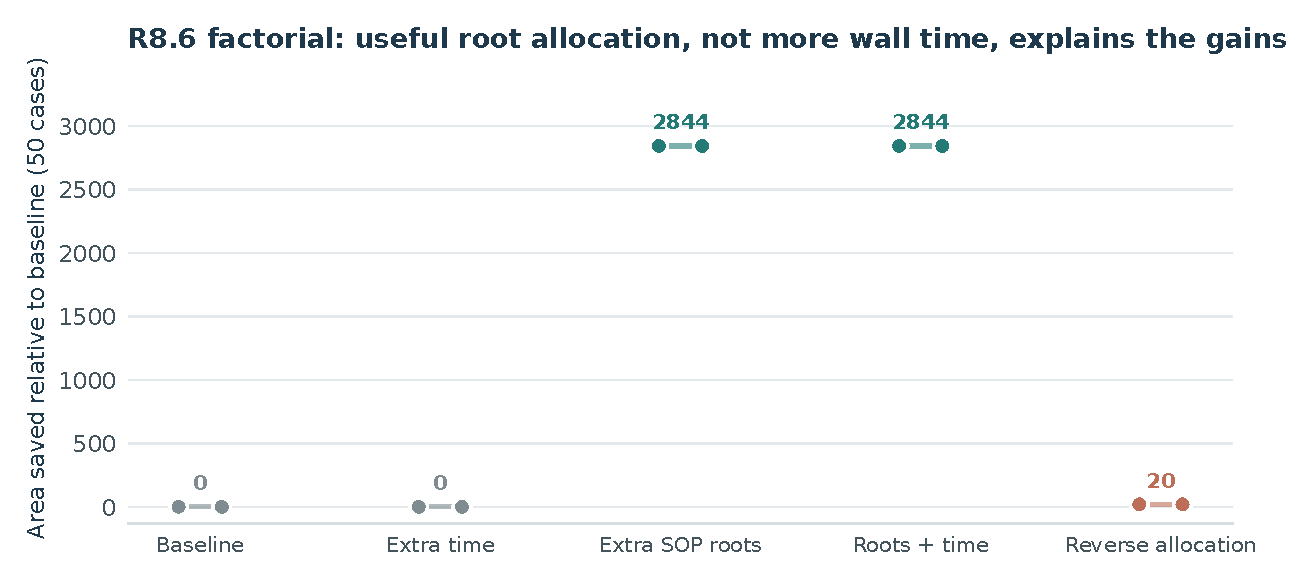
\includegraphics[width=0.99\textwidth]{../figures/04_r86_factorial.pdf}
\caption{R8.6 controlled quota allocation across 50 released cases. Points mark the two evaluator periods; identical area totals overlap in each arm. Each treatment is compared to the within-archive factorial baseline. One factor changes SOP-root quota and the other changes allowed time; the reverse-allocation treatment instead enlarges the Shannon search. This is a controlled configuration comparison, not a statement about arbitrary unseen functions.}
\label{fig:r86-factorial}
\end{figure}

\subsection{The important negative and the stopping decision}\label{the-important-negative-and-the-stopping-decision}

The reverse-allocation control is an essential counterfactual. If ``more root visits are always better'' were the adequate explanation, giving the extra quota to Shannon should have produced a similar area reduction. It did not. The result supports a targeted claim: \textbf{additional quota was valuable when given to the SOP branch of this architecture on the observed 50 cases}. It does not establish a general theorem that SOP is better than Shannon, nor guarantee monotonic savings at still larger quotas.

Runtime remains noisy. In the direct feedback, the Stage 2 median for \texttt{r86\_baseline} is 102.431 ms and for \texttt{r86\_extra\_sop} 107.818 ms in one period; \texttt{time\_reclaim} shows 95.163 ms despite identical circuit quality. These differences are not a stable law from one invocation. A 2,844-area saving has an observed search cost and should be followed by a separate robustness test, not promoted solely from the public-bank sum.

\begin{tcolorbox}[colback=ResearchBlue!6!white,colframe=ResearchSlate!55!white,boxrule=0.65pt,arc=1mm,breakable]
\textbf{Decision after R8.6:} default to the extra-SOP-root family as the promising area-oriented policy; test it on independently generated functions and explicit short-budget stress cases before calling it production-safe. That is the purpose of R8.7.
\end{tcolorbox}

\section{Round 8.7: published-case improvement is not enough to justify a universal production claim}\label{round-8.7-published-case-improvement-is-not-enough-to-justify-a-universal-production-claim}

\subsection{What the public cases can and cannot tell us}\label{what-the-public-cases-can-and-cannot-tell-us}

By the end of R8.6, repeated tuning on the released 50 cases had produced a clear candidate. The danger is no longer only a broken Boolean identity; the danger is \textbf{policy overfitting}. A root allocation chosen after inspecting a fixed finite set may be tailored to its mix of dense/sparse/cofactor/multi-output functions. Even if every recorded case passes, it does not follow that the policy improves other function families or adverse runtime limits.

R8.7 therefore freezes the candidate policies and evaluates new deterministic generated functions as a separately named data family. The feedback's \path{experiment/holdout/PROVENANCE.json} records \textbf{36 functions}, \textbf{two runs} and \textbf{three candidate policies}, plus source and executable digests. The generated cases are reproducible and can test the behavior of classes of Boolean functions that are underrepresented in the released set. They are not the evaluator's hidden cases, and a seed used for later tuning is no longer a clean unseen holdout for subsequent configurations.

\subsection{The findings were not a universal extra-SOP victory}\label{the-findings-were-not-a-universal-extra-sop-victory}

The generated-family totals for the three frozen R8.7 policies were tied in the archived comparison. In contrast, the 50 released cases retained the R8.6 extra-SOP advantage. This does \textbf{not} refute the public-case gains: it shows that a nonzero improvement on one distribution is not equivalent to broad improvement on all generated families. Most likely, the particular local opportunities and cost profiles of those constructed functions did not exercise the extra SOP work in a beneficial way. That mechanism is plausible, not uniquely established from aggregate output alone.

The tight-budget stress fixtures were an equally important negative result. Some external wall measurements on stress 001/002 ran beyond 100 ms for both baseline and extra-SOP variants, even when particular invocations of the course evaluator reported PASS. An evaluator's reported synthesis runtime, a supervisory wall stopwatch and process peak memory are \textbf{not identical instruments}. It is wrong to claim either that every run violates the official limit or that public PASS makes the implementation hard-real-time safe. The evidence supports a narrower statement: \emph{some execution paths under adverse caps deserve an early, structurally exact bypass or another conservative feasibility mechanism.}

\subsection{The next decision is a deployment policy, not a mathematical retraction}\label{the-next-decision-is-a-deployment-policy-not-a-mathematical-retraction}

The hypothesis that extra-SOP roots create additional realizable area opportunities is supported for the released 50-case bank, and those opportunities were later exploited by R9/R10. But it would be irresponsible to commit a short-limit program to additional cut search before a safe candidate is available. R9.0 retains the area-oriented policy when resources permit while addressing fast production of exact structured circuits in the special short-budget path. \textbf{The R8.7 result constrains the domain of the claim; it does not erase the optimization.}

\section{Round 9.0: a runtime-first fallback and an exact early structured-function bypass}\label{round-9.0-a-runtime-first-fallback-and-an-exact-early-structured-function-bypass}

\subsection{Why another ``faster heuristic'' would not solve the observed risk}\label{why-another-faster-heuristic-would-not-solve-the-observed-risk}

The R8.7 stress discussion highlighted the end-to-end work incurred before the ordinary BDD and mapping portfolio can emit any legal output. For certain large tables with very short budgets, a function may have a simple \emph{semantic} form even though constructing a general-purpose shared representation is expensive. Examples include constants, single literals/negated literals and affine functions over \(\mathrm{GF}(2)\).

Instead of rushing every routine, R9.0 introduces a logically separate \textbf{streaming recognition path}: while reading the full input, maintain sufficient consistency state to tell whether each output belongs to one of those restricted families. If a complete exact witness exists, construct it immediately using the three legal gate types and check its actual area and timing. If the witness does not exist or fails the target, return to the ordinary compiler; \textbf{never silently approximate the truth table}.

\subsection{The actual implementation and its correctness boundary}\label{the-actual-implementation-and-its-correctness-boundary}

The frozen \texttt{r90\_stream.hpp} defines \texttt{StreamProbe}. It maintains candidate bitsets for constants and literals, plus a per-output affine mask and validity flag. For an affine Boolean output,

\[
f(x)=c\oplus\bigoplus_{i=1}^{n}\alpha_i x_i,
\qquad \alpha_i\in\{0,1\},
\]

\(c=f(0)\) and \(\alpha_i=f(e_i)\oplus f(0)\), where \(e_i\) is the \(i\)th unit-vector input. Those \(n+1\) rows \emph{identify} an affine candidate, but do \textbf{not} prove that an arbitrary truth table is affine. The streaming verifier checks every other row against the candidate parity relation. Thus the final acceptance test is an exhaustive comparison against \textbf{all} \(2^n\) rows as they are read, not extrapolation from a handful of unit vectors.

For literals and constants, the running bitset eliminates any candidate inconsistent with a newly seen row. If all outputs are exactly implementable as simple signals or affine combinations, the builder lowers XORs using only supported gates, e.g.

\[
u\oplus v=(u\lor v)\land\neg(u\land v),
\]

shares identical subexpressions where possible, builds a legal DAG and checks the requested target delay. The code chooses an arrival-aware combination order for multiple XOR terms. The emitter still pays for every AND2, OR2 and NOT, including inversions.

The entry code in \texttt{synth.cpp} restricts this exact bypass to \textbf{\(n\ge18\)} and \textbf{\(0<L\le250\) ms} and does not skip reading the full input: it first observes all \(2^n\) truth rows, then may emit the verified exact candidate. The dimension threshold is an \textbf{engineering dispatch}, not a changed contract; the legal problem remains up to 20 inputs. The normal released cases follow the general search path, with R8.6 extra-SOP selected as the default area-oriented policy when eligible.

\subsection{What the R9.0 experiments support}\label{what-the-r9.0-experiments-support}

In a selected tight-budget stress 001 comparison, the evaluator-reported runtime for the original and new paths was \textbf{93.927 ms versus 31.581 ms}, with both marked PASS in that controlled invocation. This supports the value of the early structured path on that particular fixture. It does not prove the same benefit on unstructured random truth tables or eliminate the risk of input-reading overhead. In other stress invocations, external wall monitoring still exceeded nominal limits. The two measurement types must remain distinct.

The archived R9.0 frozen reference on the two published banks has \textbf{50/50 PASS, 50/50 target-met}, combined charged area \textbf{1,021,134} (526,135 on Stage 1 and 494,999 on Stage 2) and sum of circuit delays \textbf{2,382}. These are descriptive engineering totals, not a claimed grade. Round 9.0 is a useful \emph{runtime-first fallback}: it preserves R8.6's promising area policy in normal circumstances while adding a restricted exact path for a particularly risky class of short-budget inputs.

\subsection{What remained unsolved}\label{what-remained-unsolved}

The most valuable late-stage question was no longer whether we could change the initial representation radically. It was whether the \emph{finished} R9.0 network could benefit from one additional, strictly controlled local pass---perhaps a library of precomputed small Boolean realizations, or simply another SOP/Shannon pass---without jeopardizing feasibility. R9.1 performs exactly this comparison instead of altering multiple earlier pipeline stages simultaneously.

\section{Round 9.1: precomputed Boolean template library versus another ordinary pass}\label{round-9.1-precomputed-boolean-template-library-versus-another-ordinary-pass}

\subsection{A library is a different search mechanism, not necessarily a more powerful one}\label{a-library-is-a-different-search-mechanism-not-necessarily-a-more-powerful-one}

A truth-signature-indexed library pre-enumerates recipes for functions on 2, 3 and 4 leaves. \texttt{r91\_library.hpp} stores a bounded number of recipes per complete signature, and explicitly includes associative chains, balanced four-input combinations, MUX-like forms, XOR-like forms, majority-like forms and optional output complementation. The frozen source retains \textbf{at most 32 recipes per signature}, in a deterministic generation order. This matters: the library is not an exhaustive catalogue of minimum-area realizations under \emph{arbitrary} case-specific prices and arrival times. A recipe that is compact in generic gates need not be cheapest when a particular OR2 is expensive or when useful inversions are already live elsewhere.

A library lookup is allowed only after computing the exact cut mask. Matching that mask guarantees the local Boolean function can be realized by the recipe; actual emitted mapping and complete network cost still depend on context. A signature match by itself does not grant a free physical inverter or bypass the end-to-end timing check.

As a control, R9.1 also runs the already implemented \texttt{r84cut::rewrite} a second time in an SOP-only or Shannon-only mode. This is a valuable experimental design: it asks whether the new representation itself earns its implementation complexity, compared with spending a similar additional budget on an existing conventional method.

\subsection{Direct paired outcome: more discovered successes, less realized area benefit}\label{direct-paired-outcome-more-discovered-successes-less-realized-area-benefit}

The R9.1 native feedback supplies two periods on both banks. Each candidate passed all 50 and met all delay targets. The first and second periods agree in area values. Relative to frozen R9.0 (area 1,021,134):

\begin{longtable}[]{@{}
  >{\raggedright\arraybackslash}p{(\columnwidth - 10\tabcolsep) * \real{0.1667}}
  >{\raggedleft\arraybackslash}p{(\columnwidth - 10\tabcolsep) * \real{0.1667}}
  >{\raggedleft\arraybackslash}p{(\columnwidth - 10\tabcolsep) * \real{0.1667}}
  >{\raggedleft\arraybackslash}p{(\columnwidth - 10\tabcolsep) * \real{0.1667}}
  >{\raggedleft\arraybackslash}p{(\columnwidth - 10\tabcolsep) * \real{0.1667}}
  >{\raggedleft\arraybackslash}p{(\columnwidth - 10\tabcolsep) * \real{0.1667}}@{}}
\toprule\noalign{}
\begin{minipage}[b]{\linewidth}\raggedright
Postpass policy
\end{minipage} & \begin{minipage}[b]{\linewidth}\raggedleft
50-case total area
\end{minipage} & \begin{minipage}[b]{\linewidth}\raggedleft
Total area saved
\end{minipage} & \begin{minipage}[b]{\linewidth}\raggedleft
Improved cases
\end{minipage} & \begin{minipage}[b]{\linewidth}\raggedleft
Sum of delays
\end{minipage} & \begin{minipage}[b]{\linewidth}\raggedleft
Delay increases
\end{minipage} \\
\midrule\noalign{}
\endhead
\bottomrule\noalign{}
\endlastfoot
R9.0 frozen / off & 1,021,134 & 0 & 0 & 2,382 & --- \\
Signature-indexed library & \textbf{1,020,471} & \textbf{663} & \textbf{15} & 2,384 & 2 cases \\
Repeat Shannon & \textbf{1,020,255} & \textbf{879} & \textbf{5} & 2,381 & 0 cases \\
\textbf{Repeat SOP} & \textbf{1,019,547} & \textbf{1,587} & \textbf{8} & \textbf{2,382} & \textbf{0 cases} \\
\end{longtable}

These numbers are derived from matched per-case source CSVs, not from eyeballing a plot. They show why counting successful candidates is the wrong performance target. Library rewriting helps more individual cases than repeat-SOP, but its gains are small in magnitude and it increases the delay of two completed networks (while still meeting their own targets). Repeat-SOP helps fewer cases yet saves \textbf{more than twice} the weighted area, with no per-case delay increase on the observed set. Repeat Shannon offers a distinct, smaller benefit and a one-unit aggregate delay improvement.

The four-case lockbox study in the archive found no library area win. Because its cases and construction are narrowly defined, it should not be described as definitive proof that indexed libraries are useless. The appropriate conclusion is narrower and stronger: \textbf{under the measured budget and gate library, there is no compelling evidence to replace a simple repeat-SOP step with this particular bounded template library.}

\subsection{Why hit count and saved area answer different questions}\label{a-why-hit-count-and-saved-area-answer-different-questions}

A library lookup may recognize many reusable Boolean functions, but each winning candidate replaces a different set of \emph{live physical gates} and interacts with different fanout. Counting the number of strict improvements gives

\[
H(\pi)=\sum_{i=1}^{50}\mathbf{1}\{A_i(\pi)<A_i(\text{off})\},
\]

whereas total measured saving is

\[
S(\pi)=\sum_{i=1}^{50}\bigl(A_i(\text{off})-A_i(\pi)\bigr).
\]

Neither statistic determines the other: the first discards magnitude and the second can be dominated by a handful of expensive inputs. In the native R9.1 feedback the library wins \textbf{15} cases but saves only \textbf{663} area units; repeat-SOP wins \textbf{8} but saves \textbf{1,587}; repeat-Shannon wins \textbf{5} and saves \textbf{879}. Figure \ref{fig:r91-freq} plots the two statistics simultaneously, exposing why adopting the template library simply because it fired more often would be a poor interpretation. This comparison is valid for the same control batch; it does \textbf{not} establish that repeating SOP will always outperform an indexed library.

\begin{figure}[htbp]
\centering
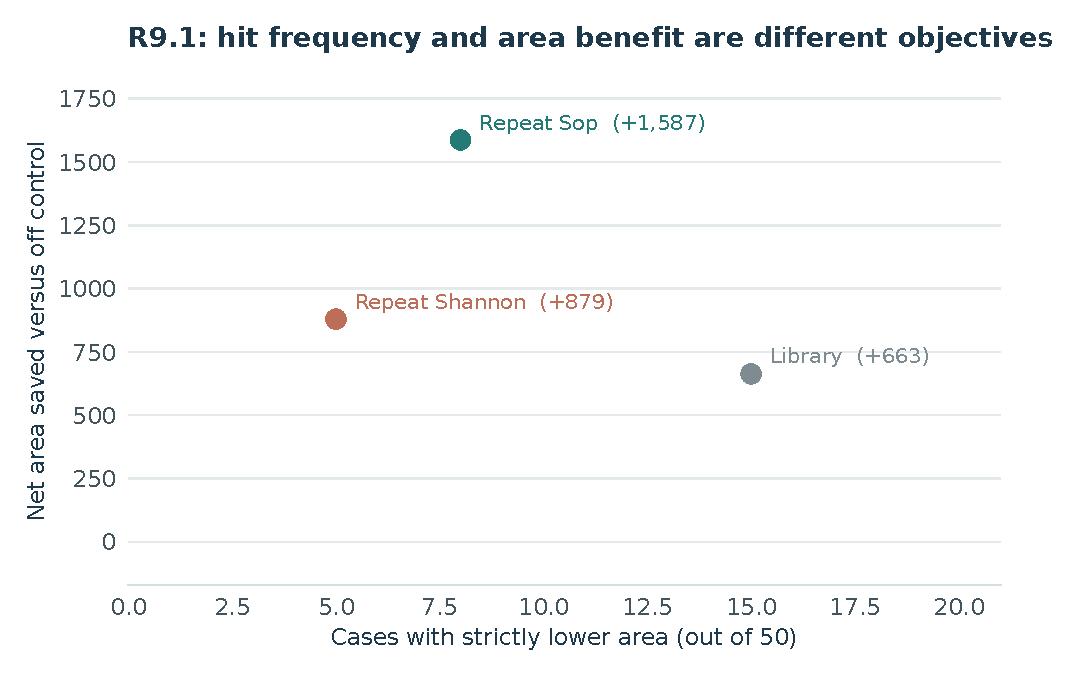
\includegraphics[width=0.90\textwidth]{../figures/05_r91_frequency_vs_magnitude.pdf}
\caption{R9.1 policy comparison on both released case banks, evaluator period 1, each relative to the same frozen off control. More cases improved does not imply more area saved.}
\label{fig:r91-freq}
\end{figure}

\subsection{How to read the runtime cost correctly}\label{how-to-read-the-runtime-cost-correctly}

A repeat pass performs real additional search. On the Stage 2 bank in the first R9.1 period, medians were approximately \textbf{104.183 ms} for R9.0, \textbf{116.551 ms} for library, \textbf{117.559 ms} for repeat-SOP and \textbf{114.906 ms} for repeat Shannon. These are within-experiment descriptive medians. They do not establish the precise deadline risk on all inputs, but they show that area improvement has a measurable computational price. That price must be restricted by a scheduling guard, rather than assuming the full final-search allowance is always safe.

\begin{tcolorbox}[colback=ResearchBlue!6!white,colframe=ResearchSlate!55!white,boxrule=0.65pt,arc=1mm,breakable]
\textbf{Decision after R9.1:} choose repeat-SOP as the final experimental postpass. Do not enable the indexed library by default. The next task is a controlled production freeze: verify that the default actually runs without a special environment variable and that disabling the pass reproduces the original R9.0 behavior.
\end{tcolorbox}

\section{Round 10.0: what was actually frozen, and why it is a defensible default}\label{round-10.0-what-was-actually-frozen-and-why-it-is-a-defensible-default}

\subsection{The source-level policy is more specific than ``use SOP twice''}\label{the-source-level-policy-is-more-specific-than-use-sop-twice}

The final \texttt{synth.cpp} first runs the inherited exact construction and its bounded R8.6 extra-SOP policy where eligible, retaining a validated incumbent. The extra \textbf{R9.1-derived} postpass is then admitted only under explicit conditions. The current frozen implementation (near lines 1841--1895) reveals the following policy contract:

\begin{enumerate}
\def\labelenumi{\arabic{enumi}.}
\tightlist
\item
  \texttt{UFUG\_R91\_POLICY} defaults to \textbf{\texttt{repeat\_sop}}, not \texttt{library} and not \texttt{off}.
\item
  The postpass is eligible only if the instance runtime limit is at least \textbf{1,000 ms}, a valid incumbent exists, and its delay already meets target.
\item
  Let \(t_{\rm used}\) be time since program launch. The allowable postpass budget is \[
  B_{\rm post}=\min\{90\text{ ms},\ 0.06L,\ 0.82L-t_{\rm used}\}.
  \] If this is below \textbf{8 ms}, no postpass is attempted.
\item
  The normal root cap is \textbf{160}, with the experimental override constrained to 20--400. The ordinary \texttt{repeat\_sop} path invokes \texttt{r84cut::rewrite} in SOP-only mode using \texttt{priority\_topq} and the specified cap. Library and repeat-Shannon exist in source for controlled experiments only.
\item
  The resulting graph is rebuilt and remeasured. It replaces the incumbent \textbf{only if} it is structurally valid, remains within target and has \textbf{strictly smaller entire-network charged area}.
\item
  Otherwise the original incumbent remains unchanged. The short-limit R9.0 exact streaming path is a separate earlier dispatch and does not pay for this optional postpass.
\end{enumerate}

The 82\% launch budget reserve is a heuristic, not an operating-system guaranteed preemption. The 90-ms maximum is an upper allowance to the extra pass; it is not an assertion that the whole program takes 90 ms or that every root visit completes in constant time. In particular, \texttt{work\_roots=160} is checked only between completed roots. The cutoff can affect the final network, which explains why a frozen source need not emit byte-identical netlists in separate wall-clock environments.

\subsection{Six-configuration freeze comparison}\label{six-configuration-freeze-comparison}

The R10.0 native feedback evaluates frozen R9.0, the R9.1 explicit SOP branch, R10.0 \texttt{off}, R10.0 \texttt{repeat\_sop} explicitly requested, R10.0 default, and the submitted copy of R10.0 default, in \textbf{two periods} on \textbf{both public banks}. This is the correct unit for verifying the release choice. In each native period:

\begin{longtable}[]{@{}
  >{\raggedright\arraybackslash}p{(\columnwidth - 8\tabcolsep) * \real{0.2000}}
  >{\raggedleft\arraybackslash}p{(\columnwidth - 8\tabcolsep) * \real{0.2000}}
  >{\raggedleft\arraybackslash}p{(\columnwidth - 8\tabcolsep) * \real{0.2000}}
  >{\raggedleft\arraybackslash}p{(\columnwidth - 8\tabcolsep) * \real{0.2000}}
  >{\raggedleft\arraybackslash}p{(\columnwidth - 8\tabcolsep) * \real{0.2000}}@{}}
\toprule\noalign{}
\begin{minipage}[b]{\linewidth}\raggedright
Candidate
\end{minipage} & \begin{minipage}[b]{\linewidth}\raggedleft
Complete cases
\end{minipage} & \begin{minipage}[b]{\linewidth}\raggedleft
Target-met
\end{minipage} & \begin{minipage}[b]{\linewidth}\raggedleft
Total Area
\end{minipage} & \begin{minipage}[b]{\linewidth}\raggedleft
Total circuit Delay
\end{minipage} \\
\midrule\noalign{}
\endhead
\bottomrule\noalign{}
\endlastfoot
Frozen R9.0 & 50/50 & 50/50 & 1,021,134 & 2,382 \\
R10.0 postpass \texttt{off} & 50/50 & 50/50 & 1,021,134 & 2,382 \\
R9.1 explicit repeat-SOP & 50/50 & 50/50 & 1,019,547 & 2,382 \\
R10.0 explicit repeat-SOP & 50/50 & 50/50 & 1,019,547 & 2,382 \\
\textbf{R10.0 default} & \textbf{50/50} & \textbf{50/50} & \textbf{1,019,547} & \textbf{2,382} \\
R10.0 submission default & 50/50 & 50/50 & 1,019,547 & 2,382 \\
\end{longtable}

The \texttt{off} arm restoring the R9.0 area/delay is an important \textbf{negative control}. The explicit-vs-default comparison establishes the chosen behavior under the evaluation setup; the submission-vs-research comparison checks packaging consistency. The frozen R10.0 source translation unit and the copy used for the reproducibility study have the same complete SHA-256 \texttt{8c863f1a1c9555ae571948a0424c25642c29c9a9f98f1f3e5f193c6b20f5b15d}.

\subsection{Only eight cases drive the 1,587-area improvement}\label{only-eight-cases-drive-the-1587-area-improvement}

Per-case, frozen R10.0 improves \textbf{8 out of 50} released instances and ties \textbf{42 out of 50} relative to R9.0, with \textbf{no area regressions} and \textbf{no per-case delay changes} in both native periods. The exact improvement cases and charged-area savings are:

\begin{longtable}[]{@{}lr@{}}
\toprule\noalign{}
Bank / case & Area saved \\
\midrule\noalign{}
\endhead
\bottomrule\noalign{}
\endlastfoot
Stage 1 / 010 & 298 \\
Stage 1 / 012 & 250 \\
Stage 1 / 016 & 5 \\
Stage 2 / 003 & 150 \\
Stage 2 / 005 & \textbf{752} \\
Stage 2 / 012 & 2 \\
Stage 2 / 023 & 125 \\
Stage 2 / 024 & 5 \\
\textbf{Combined} & \textbf{1,587} \\
\end{longtable}

Stage 2 / 005 contributes \textbf{752/1,587 = 47.39\%} of the observed saving. This concentration matters in two ways. First, median improvement per case is zero, so a statement such as ``the optimizer improves the typical case by 0.155\%'' is false. The 0.155\% is a \emph{weighted area-total comparison}, not a typical-instance outcome. Second, one or two case-sensitive opportunities could dominate future aggregate totals as well. This does not invalidate the improvement, but it makes per-case detail and holdout/generalization discussion indispensable.

The reduction from 1,021,134 to 1,019,547 is about \textbf{0.1554\%} relative to the R9.0 aggregate; it is deliberately modest. The value of this last round lies in a \emph{verified strict-improvement postpass} plus preserved target feasibility and rollback---not in claiming a radical new Boolean synthesis theory.

\subsection{\texorpdfstring{16.3a What the \emph{size distribution} adds to the R10.0 summary}{16.3a What the size distribution adds to the R10.0 summary}}\label{a-what-the-size-distribution-adds-to-the-r10.0-summary}

The eight improvements are not close in magnitude. Their exact contributions are \textbf{752, 298, 250, 150, 125, 5, 5, and 2} (sum 1,587), in descending order. Thus a single Stage 2 case supplies \textbf{47.39\%} of the incremental gain; the five largest supply \textbf{1,575 of 1,587}, or \textbf{99.24\%}. The three smallest wins total only 12 units. They should not be deleted from the record merely because they are small: they verify that the optimization is not logically limited to large step changes, but neither do they justify characterizing the method as a broadly effective optimization on every input.

A measure of the concentration is

\[
C_k=\frac{\sum_{j=1}^{k}g_{(j)}}{\sum_{j=1}^{8}g_{(j)}},
\qquad g_{(1)}\ge\cdots\ge g_{(8)}>0,
\]

with \(C_1=0.4739\) and \(C_5=0.9924\). These are descriptive finite-benchmark statistics, not inferred population probabilities. Figure \ref{fig:r100-sparse} uses exact area units so the 2-unit and 5-unit changes remain legible instead of disappearing in a million-unit total.

\begin{figure}[htbp]
\centering
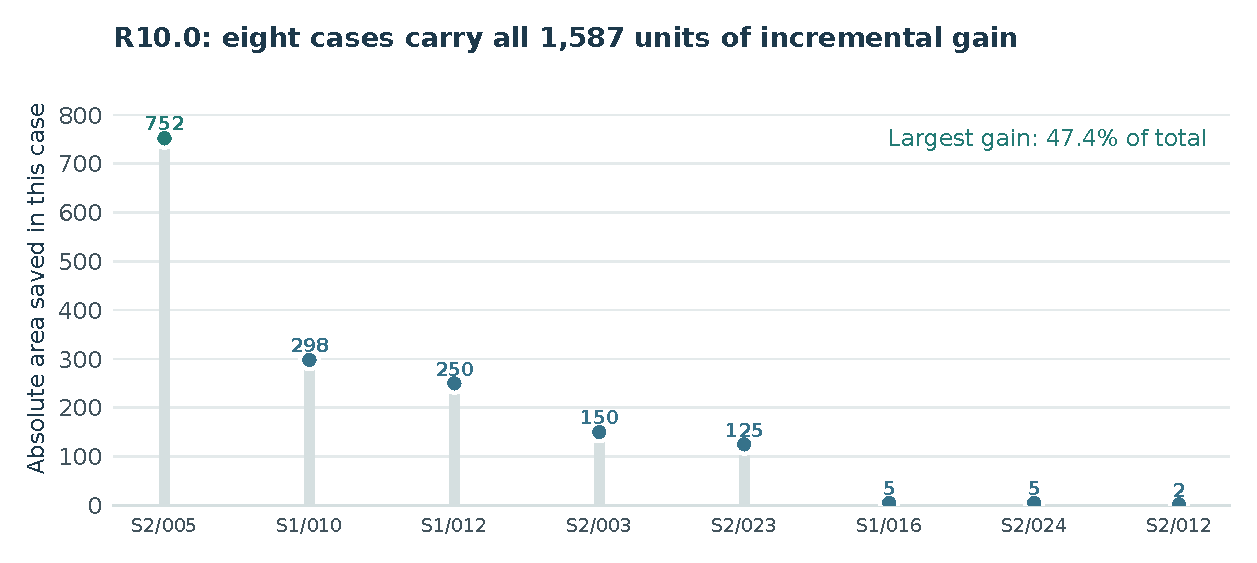
\includegraphics[width=0.98\textwidth]{../figures/06_r100_sparse_case_gains.pdf}
\caption{R10.0 final default versus R9.0 frozen in the directly decoded first-period official feedback. All 42 other cases have zero area change, no area regression is observed, and circuit delays are unchanged. S1/S2 designate the two case banks, not two algorithms.}
\label{fig:r100-sparse}
\end{figure}

\subsection{The runtime tradeoff is not monotonically favorable}\label{the-runtime-tradeoff-is-not-monotonically-favorable}

The direct feedback shows different effects by case and run order. Comparing the geometric per-case runtime ratios for R10.0 to R9.0 on the native pair gives approximately \textbf{0.961} in one period and \textbf{1.075} in the reverse period. A value below 1 means the R10 candidate was geometrically faster on the observed paired cases despite performing nominally more search; a value above 1 means it was slower. Runtime scheduling, OS contention and a clock-gated portfolio all contribute variability. Without a controlled trace of every candidate's clock gate, neither number can be generalized as ``the SOP postpass is always 3.9\% faster'' or ``always 7.5\% slower.''

The source establishes a reserve rule and fallback; the feedback establishes released-case validity and observed tradeoffs. Neither constitutes a formal upper bound on all \(T_{\rm synth}\) or RAM on hidden instances. This difference between \emph{observed successful deployability} and \emph{proven bounded runtime} must remain visible in the final project narrative.

\begin{tcolorbox}[colback=ResearchBlue!6!white,colframe=ResearchSlate!55!white,boxrule=0.65pt,arc=1mm,breakable]
\textbf{Decision after R10.0:} freeze the complete default and its source hash. Retain R9.0 as the runtime-first comparator/fallback. Do not promote speculative postpass variants without showing an equal-or-better outcome under comparable controls.
\end{tcolorbox}

\section{Round 10.1: a reasonable runtime hypothesis that was not supported by the quality evidence}\label{round-10.1-a-reasonable-runtime-hypothesis-that-was-not-supported-by-the-quality-evidence}

\subsection{The question: can a smaller postpass recover the useful part of a concentrated gain?}\label{the-question-can-a-smaller-postpass-recover-the-useful-part-of-a-concentrated-gain}

Because only eight cases benefit from the repeat-SOP pass, it is tempting to reduce its root cap or nominal allowance and hope to preserve almost all area savings with less synthesis time. This is a sensible \emph{research question}. It is not yet a justified optimization: profitable roots might occur late in the ranked set, and one expensive case may dominate the aggregate payoff. The root cap is a search-space selection rule, not simply a linear throttle on CPU milliseconds.

R10.1 keeps the frozen R10.0 comparator and tests a default identity, root caps \textbf{80} and \textbf{40}, and an allowance of \textbf{45 ms}. The source also retains a trial submission control. Native feedback again covers 50 cases in two periods; all variants pass all released cases and meet their targets.

\subsection{Recomputed native results}\label{recomputed-native-results}

\begin{longtable}[]{@{}
  >{\raggedright\arraybackslash}p{(\columnwidth - 8\tabcolsep) * \real{0.2000}}
  >{\raggedleft\arraybackslash}p{(\columnwidth - 8\tabcolsep) * \real{0.2000}}
  >{\raggedleft\arraybackslash}p{(\columnwidth - 8\tabcolsep) * \real{0.2000}}
  >{\raggedleft\arraybackslash}p{(\columnwidth - 8\tabcolsep) * \real{0.2000}}
  >{\raggedleft\arraybackslash}p{(\columnwidth - 8\tabcolsep) * \real{0.2000}}@{}}
\toprule\noalign{}
\begin{minipage}[b]{\linewidth}\raggedright
Policy
\end{minipage} & \begin{minipage}[b]{\linewidth}\raggedleft
Total Area
\end{minipage} & \begin{minipage}[b]{\linewidth}\raggedleft
Area \emph{worse} than R10.0
\end{minipage} & \begin{minipage}[b]{\linewidth}\raggedleft
Circuit delay difference
\end{minipage} & \begin{minipage}[b]{\linewidth}\raggedleft
Cases that lose area vs frozen R10
\end{minipage} \\
\midrule\noalign{}
\endhead
\bottomrule\noalign{}
\endlastfoot
R10.0 frozen & \textbf{1,019,547} & 0 & 0 & 0 \\
R10.1 default identity & 1,019,547 & 0 & 0 & 0 \\
Root cap 80 & 1,020,149 & \textbf{+602} & 0 & 6 \\
Root cap 40 & 1,020,555 & \textbf{+1,008} & 0 & 6 \\
Nominal budget 45 ms & 1,019,788 & \textbf{+241} & 0 & 1 \\
\end{longtable}

The two feedback periods agree on these area totals and number of regressing cases. On the Stage 2 bank, the 45-ms limit loses 241 area units on a single case. Root cap 40 loses 352 area units across two Stage 1 cases and 656 across four Stage 2 cases. Cap 80 loses 212 and 390 respectively. No circuit-delay benefit compensates for these losses.

Measured median runtime also does not offer a clean cross-case dominance result. Shrinking the nominal cap changes some observed medians in either direction depending on the bank and repeat, and the amount of actual local work may already be below the earlier allowance. A smaller \emph{ceiling} is not equivalent to a demonstrated reduced cost on every case. This is precisely the danger that R8.3--R8.6 taught us to distinguish.

\begin{tcolorbox}[colback=ResearchBlue!6!white,colframe=ResearchSlate!55!white,boxrule=0.65pt,arc=1mm,breakable]
\textbf{Decision after R10.1: No-Go.} Preserve R10.0 as final. This negative experiment does not prove 160 roots or a 90-ms ceiling globally optimal. It establishes that \textbf{these tested reductions did not retain the observed released-case benefit or show a sufficiently robust compensation in runtime}. Having a defensible stopping decision is part of the research, not an embarrassment to hide.
\end{tcolorbox}

\section{\texorpdfstring{18. The official cross-stage comparison: three \emph{different} questions, not one misleading scoreboard}{18. The official cross-stage comparison: three different questions, not one misleading scoreboard}}\label{the-official-cross-stage-comparison-three-different-questions-not-one-misleading-scoreboard}

\subsection{Why these three programs must be separated}\label{why-these-three-programs-must-be-separated}

The final assignment asks for the \emph{actually submitted} Stage 1 method and the proposed Stage 2 method on \textbf{both released banks}. We therefore treat \textbf{Z1} (Zeyun DU's submitted Stage 1 implementation) versus \textbf{S100} (the frozen R10.0 Stage 2 implementation) as the \emph{officially relevant method comparison}. Independently, \textbf{J51} is Jincan LI's frozen Stage 1 R5.1 research implementation, a technically important alternate research line whose own trial log and R6 extensions contributed the ideas and implementation lineage underlying Stage 2. Treating J51 as non-existent because it was not administratively submitted would falsify the history; treating its output as the submitted Stage 1 method would falsify the project contract.

A new same-directory, same-evaluator study uses an interleaved/reversed order in \textbf{two periods}, over both 25-case banks, running all three source-frozen methods: \textbf{2 periods × 2 banks × 25 cases × 3 programs = 300 case-program invocations}. The input SHA-256 and source fingerprints are recorded in the reproduction bundle; Z1, J51 and S100 use \textbf{different source hashes}, not labels attached to the same executable. The table below is the direct result of \texttt{06\_reproducibility/matched\_batch/stage\{1,2\}\_run\{1,2\}\_\{Z1,J51,S100\}.csv} and independently cross-checked against \texttt{02\_analysis/matched\_summary.csv}.

\begin{longtable}[]{@{}
  >{\raggedright\arraybackslash}p{(\columnwidth - 12\tabcolsep) * \real{0.1429}}
  >{\raggedright\arraybackslash}p{(\columnwidth - 12\tabcolsep) * \real{0.1429}}
  >{\raggedleft\arraybackslash}p{(\columnwidth - 12\tabcolsep) * \real{0.1429}}
  >{\raggedleft\arraybackslash}p{(\columnwidth - 12\tabcolsep) * \real{0.1429}}
  >{\raggedleft\arraybackslash}p{(\columnwidth - 12\tabcolsep) * \real{0.1429}}
  >{\raggedleft\arraybackslash}p{(\columnwidth - 12\tabcolsep) * \real{0.1429}}
  >{\raggedleft\arraybackslash}p{(\columnwidth - 12\tabcolsep) * \real{0.1429}}@{}}
\toprule\noalign{}
\begin{minipage}[b]{\linewidth}\raggedright
Bank / repeat
\end{minipage} & \begin{minipage}[b]{\linewidth}\raggedright
Method
\end{minipage} & \begin{minipage}[b]{\linewidth}\raggedleft
PASS
\end{minipage} & \begin{minipage}[b]{\linewidth}\raggedleft
Target-met
\end{minipage} & \begin{minipage}[b]{\linewidth}\raggedleft
\textbf{Area on PASS rows}
\end{minipage} & \begin{minipage}[b]{\linewidth}\raggedleft
\textbf{Delay on PASS rows}
\end{minipage} & \begin{minipage}[b]{\linewidth}\raggedleft
Median synthesis time (ms)
\end{minipage} \\
\midrule\noalign{}
\endhead
\bottomrule\noalign{}
\endlastfoot
Stage 1 / 1 & Z1 & 25/25 & 25/25 & 589,023 & 1,271 & 605.748 \\
Stage 1 / 1 & J51 & 25/25 & 25/25 & 529,014 & 1,167 & 61.360 \\
Stage 1 / 1 & S100 & 25/25 & 25/25 & \textbf{525,582} & 1,212 & 193.699 \\
Stage 2 / 1 & Z1 & 25/25 & 25/25 & 555,221 & 1,128 & 603.776 \\
Stage 2 / 1 & J51 & \textbf{24/25} & \textbf{24/25} & 506,754 & 1,065 & 36.929 \\
Stage 2 / 1 & S100 & 25/25 & 25/25 & \textbf{493,965} & 1,170 & 130.707 \\
Stage 1 / 2 & Z1 & 25/25 & 25/25 & 589,023 & 1,271 & 609.505 \\
Stage 1 / 2 & J51 & 25/25 & 25/25 & 529,014 & 1,167 & 51.627 \\
Stage 1 / 2 & S100 & 25/25 & 25/25 & \textbf{525,677} & 1,212 & 220.532 \\
Stage 2 / 2 & Z1 & 25/25 & 25/25 & 556,168 & 1,128 & 604.088 \\
Stage 2 / 2 & J51 & \textbf{24/25} & \textbf{24/25} & 506,754 & 1,065 & 36.835 \\
Stage 2 / 2 & S100 & 25/25 & 25/25 & \textbf{494,206} & 1,170 & 123.591 \\
\end{longtable}

\textbf{Interpret the denominator, not just the total.} J51's 506,754 on the second bank covers only \textbf{24 passing cases}; it is \emph{not} a 25-case total and cannot be placed in a simple 50-case ranking beside two 50/50-pass methods. The failure is \textbf{Stage 2 / case\_016} under its short runtime cap, and the observed low median for the 24 successes cannot excuse an invalid result on the excluded case. The default Z1 and S100 have 50/50 PASS and 50/50 target-met in both periods. Their successful-case sums, unlike J51's, cover identical complete case sets.

In repeat 1, the legitimate Z1--S100 total-area contrast is

\[
A_{\mathrm{Z1}}=589{,}023+555{,}221=1{,}144{,}244,
\quad A_{\mathrm{S100}}=525{,}582+493{,}965=1{,}019{,}547,
\]

\[
A_{\mathrm{Z1}}-A_{\mathrm{S100}}=124{,}697,
\qquad \frac{124{,}697}{1{,}144{,}244}\approx 10.90\%.
\]

In repeat 2, the respective sums are \textbf{1,145,191 and 1,019,883}, a \textbf{125,308} unit difference. These improvements are strong \emph{released-case aggregate} results. The time medians differ substantially, but they represent a different cost dimension, so no single scalar combined winner is asserted without an official utility formula or explicit constraints.

\subsection{The key reversal: a lower weighted total despite losing more individual cases}\label{the-key-reversal-a-lower-weighted-total-despite-losing-more-individual-cases}

The first period contains an instructive ranking reversal. Relative to Z1, S100 has \textbf{lower area on 18 of 50 individual cases and higher area on 32}, with \textbf{zero ties}. The Stage 1 split is 9 wins versus 16 losses; the Stage 2 split is also 9 versus 16. Yet S100 saves 124,697 area units across those 50 cases. There is no contradiction:

\[
\sum_{i=1}^{50}\bigl(A_i(\mathrm{S100})-A_i(\mathrm{Z1})\bigr)
= \sum_{i:\Delta_i<0}\Delta_i+\sum_{i:\Delta_i>0}\Delta_i,
\quad\Delta_i=A_i(\mathrm{S100})-A_i(\mathrm{Z1}).
\]

\textbf{Magnitude}, not the sign count, determines this sum. The median relative change across the 50 cases is actually \textbf{+3.69\%} (S100 area worse for the median case). This fact must accompany the aggregate improvement, not be hidden behind it. Examples make the point concrete:

\begin{itemize}
\tightlist
\item
  \textbf{Stage 2 / 005:} Z1 emits area \textbf{142,405}, delay \textbf{40}. S100 emits area \textbf{102,889}, delay \textbf{68}. Area improves by \textbf{39,516}, while circuit delay increases by \textbf{28}. Both meet their \emph{own case's} reported target. This is a feasible \textbf{area-versus-delay trade}, not strict Pareto dominance.
\item
  \textbf{Stage 2 / 002:} Z1 has area \textbf{50,694}, delay \textbf{77}. S100 has area \textbf{58,697}, delay \textbf{68}. Here the \emph{sign reverses}: S100 pays \textbf{8,003 more area} to remove \textbf{nine delay units}. The optimization direction depends on the realized network, allowed slack, mapping choices and candidate policy.
\item
  \textbf{Stage 1 / 007 and 025:} S100 saves \textbf{28,531} and \textbf{25,957} area units respectively, explaining why the Stage 1 bank as a whole improves even though 16 of its 25 cases become larger.
\end{itemize}

Thus the correct finding is: \textbf{on the measured 50-case benchmark, the proposed Stage 2 solver finds much cheaper networks for a minority of high-impact inputs while remaining valid across all 50; it is not uniformly area-superior to the submitted Stage 1 solver.} The comparison also concerns \textbf{two distinct code lineages}, not a single isolated patch. It cannot attribute all 124,697 units to one SOP pass or to the cut engine alone.

\subsection{The magnitude distribution behind the apparent ranking reversal}\label{a-the-magnitude-distribution-behind-the-apparent-ranking-reversal}

The paired study has \textbf{18 positive per-case savings}, totaling \textbf{160,696}, and \textbf{32 negative per-case savings}, totaling \textbf{-35,999}; their net is \textbf{+124,697}. The five largest improvements together save \textbf{129,623}, exceeding the final net saving after all the regressions. This is the appropriate explanation for why the average across areas improves while a majority of individual cases become larger. It is also a warning about \emph{which} aggregate is used: summing raw area units weights naturally large circuits more heavily; taking the median relative change instead gives the typical \textbf{percentage} change on one benchmark case, which is \textbf{+3.69\% in Stage 2 area} (worse for S100 versus Z1).

\begin{figure}[htbp]
\centering
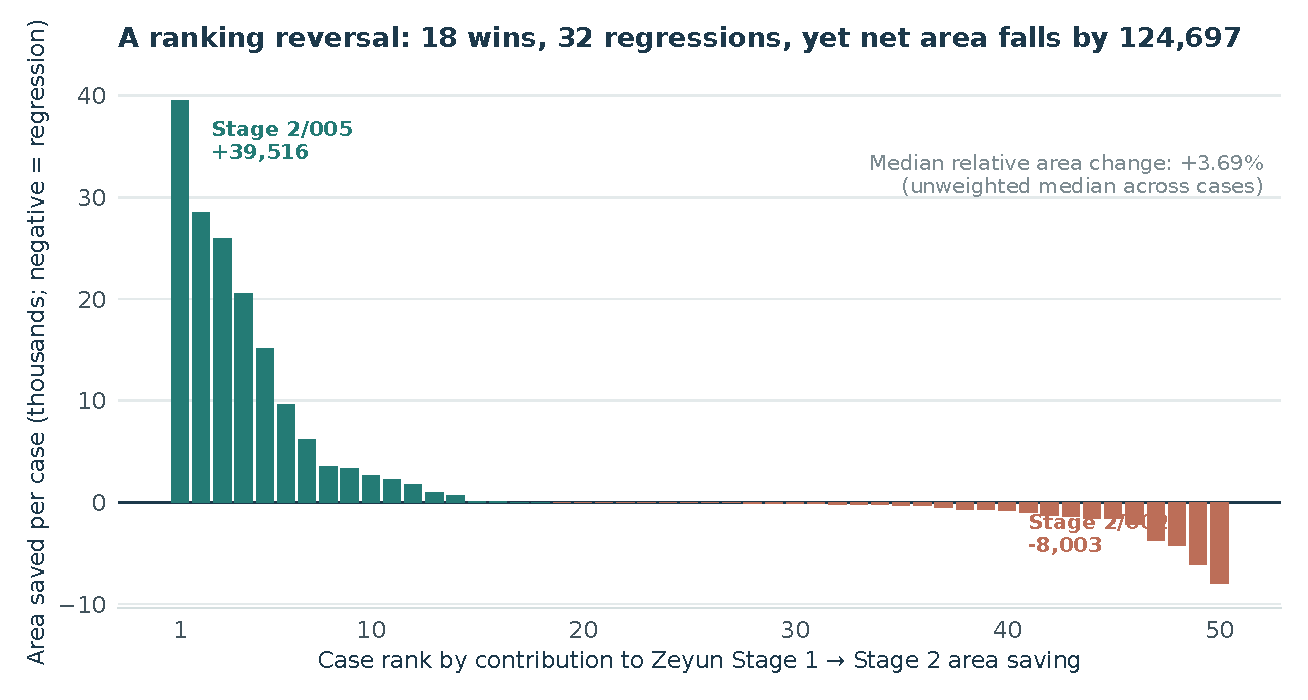
\includegraphics[width=0.98\textwidth]{../figures/07_matched_area_rank_reversal.pdf}
\caption{S100 versus Z1: the complete 50-case distribution of area savings from the independently executed first period, sorted by magnitude. Positive bars mean the Stage 2 implementation has smaller area; negative bars are genuine regressions, not invalid cases. Both programs pass all 50.}
\label{fig:ranking-reversal}
\end{figure}

The ranked cumulative sum \(C(k)=\sum_{j=1}^{k}(A_{\mathrm{Z1},(j)}-A_{\mathrm{S100},(j)})\) in Figure \ref{fig:cumulative-contribution} makes the tension visible from another angle: the positive contributors raise it to \textbf{160,696}, and 32 regressions reduce it to \textbf{124,697}. The curve does \emph{not} trace chronological training progress; its order is chosen retrospectively by observed contribution. It therefore describes concentration, not a deployable selection policy.

\begin{figure}[htbp]
\centering
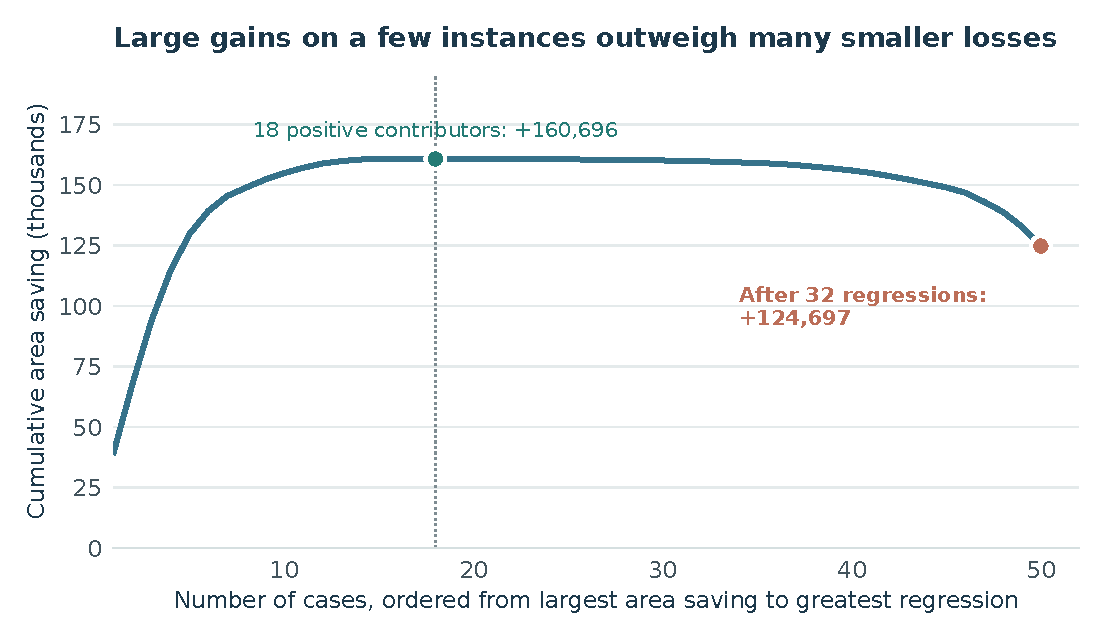
\includegraphics[width=0.88\textwidth]{../figures/08_matched_cumulative_contribution.pdf}
\caption{Cumulative per-case area contributions, ordered from most favorable to least favorable for S100. The two endpoints correspond to the 18 improvements and the full 50 cases respectively.}
\label{fig:cumulative-contribution}
\end{figure}

\subsection{Where Jincan's independent Stage 1 line fits}\label{where-jincans-independent-stage-1-line-fits}

J51 is not dispensable merely because Z1 was submitted. Against Z1 in repeat 1, J51 has lower area on \textbf{15 of their 49 jointly passing cases} and still saves \textbf{106,829} area units on that matched common-case set. Its complete Stage 1 bank has area 529,014 versus Z1's 589,023, and its median synthesis runtime there is much shorter. These are substantive algorithmic and implementation contributions, consistent with its independent Stage 1 development record. However, J51's \textbf{Stage 2 / 016 FAIL} exposes the limit that R7 addressed: a capable high-quality synthesis search can still fail the \textbf{actual resource contract}. The failure is not cured by excluding the case or replacing it with an estimated area.

The scientifically useful comparison is therefore \textbf{triangular}:

\begin{enumerate}
\def\labelenumi{\arabic{enumi}.}
\tightlist
\item
  \textbf{Z1 → S100}: official Stage 1 submitted method versus final Stage 2 method, under the same released case set.
\item
  \textbf{J51 → S100}: the development pathway from independent Stage 1 research to a new Stage 2 engineering solution, including a failure mode repaired in Stage 2.
\item
  \textbf{R9.0 → R10.0}: a much narrower frozen-source \textbf{within-lineage ablation}, identifying the marginal effect of the final optional SOP pass on released cases.
\end{enumerate}

These answer different questions; none may substitute for another. The final report can emphasize the mandated Z1→S100 comparison without erasing J51's technical ancestry.

\subsection{Same-source changes across periods are an experimental fact}\label{same-source-changes-across-periods-are-an-experimental-fact}

In the matched independent repeat, S100's total area increases by \textbf{95} on Stage 1 / 012 and \textbf{241} on Stage 2 / 005; Z1 adds \textbf{947} on Stage 2 / 021. The same respective source hashes and input hashes were used. Circuit delay totals are unchanged. This is evidence of \textbf{output sensitivity across observed runtime conditions}, not source-version drift. Both engines contain clock-aware candidate stopping/selection, so differing candidate trajectories are plausible. There is no root-by-root production trace demonstrating \emph{exactly which} deadline or branch caused each difference. A correct research log records the observed difference and candidate-clock explanation as \textbf{hypothesis}, not as a proved causal trace.

The native R10.0 feedback was a \emph{different controlled batch} in which both periods happened to return area 1,019,547 for the default. That agreement cannot be silently imposed on the independent three-method test. Both observations are valid within their own recorded conditions.

\begin{tcolorbox}[colback=ResearchBlue!6!white,colframe=ResearchSlate!55!white,boxrule=0.65pt,arc=1mm,breakable]
\textbf{Decision from the matched study:} maintain two separate Stage 1 accounts; use Z1 versus S100 to satisfy the assignment and J51 versus S100 to explain genuine technical development. Keep per-case area, delay, time and target status together. Never infer program superiority from the area summed only over successes if the success sets differ.
\end{tcolorbox}

\section{Fixed-incumbent experiment: what a two-pass order hypothesis actually predicts}\label{fixed-incumbent-experiment-what-a-two-pass-order-hypothesis-actually-predicts}

\subsection{Why the previous R8.5 evidence did not isolate pass order}\label{why-the-previous-r8.5-evidence-did-not-isolate-pass-order}

R8.5 changed ordering and sometimes reclaimed time and modified quota, so its production comparison could not isolate the algebraic effect of order. A clean diagnostic must hold \textbf{the starting network} fixed and also make the amount of work countable. The additional reproduction study \texttt{02\_analysis/FIXED\_GRAPH\_EXPERIMENT.md} does this; it must be distinguished from the historical released-case benchmarking because the six test cases were \textbf{purposively chosen after inspecting results}, not selected as an untouched random sample.

For each of six selected inputs, R10.0 with its optional final postpass explicitly disabled created and saved \textbf{one initial incumbent DAG}. Four experimental arms begin with that exact frozen graph: SOP only (\textbf{P}), Shannon only (\textbf{H}), SOP then Shannon (\textbf{PH}) and Shannon then SOP (\textbf{HP}). Both two-pass arms use the same frozen \texttt{r84cut::rewrite} code, the same Top-Q/root-ranking policy, and \textbf{160 visited roots per pass}. The emergency 60-second ceiling was never triggered, so truncation cannot explain this particular order comparison. Every pass accepts a replacement only if it preserves the function, remains target-feasible and strictly reduces global live-gate area.

\subsection{The mathematical reason pass order need not commute}\label{the-mathematical-reason-pass-order-need-not-commute}

A rewrite operator is state-dependent: its current root set, cut frontiers, future fanouts and canonical hash lookups are functions of its \textbf{input graph}, not just the output Boolean function. Therefore, in general,

\[
P(H(G))\not\cong H(P(G)),
\]

where \(\cong\) denotes structural DAG equivalence, although both graphs satisfy \(F_{P(H(G))}=F_{H(P(G))}=F_G\) provided all individual substitutions are correct. Moreover, if both operators are strict-area-decreasing when they accept a candidate, then

\[
A(P(G))\le A(G),\quad A(H(G))\le A(G),
\quad A(P(H(G)))\le A(H(G)),\quad A(H(P(G)))\le A(P(G)).
\]

These inequalities bound the \emph{admitted} output area but do not order the two compositions against each other. The search landscape changes after the first transformation: the same formal Boolean function can be realized with different shared subgraphs, arrival times and feasible cut choices.

\subsection{What the verified fixed-graph evidence says}\label{what-the-verified-fixed-graph-evidence-says}

All \textbf{24 final arms} and the six seed outputs were independently simulated against the full source truth tables; the experiments have retained input/netlist SHA-256 fingerprints. Among the six selected graphs, \textbf{PH wins three}, \textbf{HP wins one} and \textbf{two tie}. The sign reversal is observable on individual fixed incumbents:

\begin{longtable}[]{@{}
  >{\raggedright\arraybackslash}p{(\columnwidth - 10\tabcolsep) * \real{0.1667}}
  >{\raggedleft\arraybackslash}p{(\columnwidth - 10\tabcolsep) * \real{0.1667}}
  >{\raggedleft\arraybackslash}p{(\columnwidth - 10\tabcolsep) * \real{0.1667}}
  >{\raggedleft\arraybackslash}p{(\columnwidth - 10\tabcolsep) * \real{0.1667}}
  >{\raggedleft\arraybackslash}p{(\columnwidth - 10\tabcolsep) * \real{0.1667}}
  >{\raggedright\arraybackslash}p{(\columnwidth - 10\tabcolsep) * \real{0.1667}}@{}}
\toprule\noalign{}
\begin{minipage}[b]{\linewidth}\raggedright
Fixed seed
\end{minipage} & \begin{minipage}[b]{\linewidth}\raggedleft
Area before
\end{minipage} & \begin{minipage}[b]{\linewidth}\raggedleft
Area after PH
\end{minipage} & \begin{minipage}[b]{\linewidth}\raggedleft
Area after HP
\end{minipage} & \begin{minipage}[b]{\linewidth}\raggedleft
Delay of compared outputs
\end{minipage} & \begin{minipage}[b]{\linewidth}\raggedright
Interpretation
\end{minipage} \\
\midrule\noalign{}
\endhead
\bottomrule\noalign{}
\endlastfoot
Stage 2 / 005 & 103,641 & \textbf{102,471} & 102,716 & 68 & SOP-first better by 245 on this frozen graph. \\
Stage 2 / 003 & 15,773 & 15,585 & \textbf{15,575} & 65 & Shannon-first better by 10 on this frozen graph. \\
\end{longtable}

The actual full source is \path{06_reproducibility/scripts/fixed_order.cpp}; the launcher, detailed per-pass metrics and netlist verifications are in \path{06_reproducibility/scripts/fixed_order.py} and \path{fixed_batch/fixed_order.csv}. The contrast demonstrates \textbf{path dependence under fixed input DAG and root count}, not an overall superiority of one order across unseen cases. That distinction is important: equal quota controls one dimension of search effort; it does not make every pass have equal numbers of cuts, candidate materializations or CPU instructions.

This mechanism experiment closes an attribution gap in R8.5: it proves by controlled counterexample that the two pass orders can produce different final network areas. It does \emph{not} identify one universally better production order. The conservative source selection of R10.0, rather than speculative composition of every pass family, remains justified.

\section{Reconstructing the final synthesis algorithm as a complete executable pipeline}\label{reconstructing-the-final-synthesis-algorithm-as-a-complete-executable-pipeline}

A trial log should end with a clear account of \textbf{what the frozen solution actually does}, not only how its experiments are named. The following is a source-backed schematic of the frozen R10.0 translation unit and its included headers, with optional research branches separated from the shipped default. Individual candidate selection and timing guards are simplified in notation here; for literal thresholds consult the source-level descriptions in Sections 12, 14 and 16.

\begin{verbatim}
synthesize(instance):
    read n, m, gate areas/delays, delay target, optional resource limits
    read the complete 2^n-row, m-output truth table
    if (n >= 18 and 0 < runtime_limit <= 250 ms):
         verify streaming-identified constant/literal/affine forms on ALL rows
         if a legal, target-feasible exact network is constructed:
              emit it and finish
    incumbent = Stage-1-derived multi-candidate Boolean/network synthesis
    validate/prune/measure entire output-reachable AND2/OR2/NOT DAG
    if documented R8.6 eligibility and budget guards hold:
         from the SAME frozen incumbent evaluate bounded Shannon and SOP
         cut-resynthesis branches under the selected root-allocation policy
         keep a valid candidate only if its complete cost is preferred
    if runtime_limit >= 1000 ms and incumbent is valid and target-feasible:
         available = min(90 ms, 0.06*runtime_limit,
                         0.82*runtime_limit - elapsed_since_launch)
         if available >= 8 ms:
              trial = SOP-only priority_topq rewrite on incumbent
                      (normal cap 160 visited roots)
              if trial valid AND trial delay <= target
                     AND trial entire-DAG area < incumbent area:
                   incumbent = trial
    emit the legal topological netlist of incumbent
\end{verbatim}

This is an \textbf{algorithmic summary}, not an assertion of all-source formal verification. Its architecture explains several otherwise scattered research decisions:

\begin{itemize}
\tightlist
\item
  The Stage 1 machinery supplies an exact legal construction and diversified mapping rather than hoping a cut optimizer can reconstruct the entire function from scratch.
\item
  The incumbent-first discipline learned in R7 ensures optional improvements do not replace a valid circuit with a partially built or rejected candidate.
\item
  R8.1's cut truth signatures ensure local semantic equality while liveness pruning and whole-DAG scoring prevent incorrect area accounting.
\item
  R8.3--R8.6 control which candidate roots are searched, rather than assuming elapsed time alone measures useful work.
\item
  R9.0 recognizes exact cheap structure early on a narrowly specified short-budget branch; ordinary cases remain in the general synthesis path.
\item
  The adopted R10.0 extra postpass is \textbf{monotone in admitted area for a fixed incumbent}: if it fires and its result is accepted, area strictly decreases and target feasibility is retained. It is \textbf{not} monotone across independent whole-program invocations in clock-dependent search, nor a guarantee of universal runtime dominance.
\end{itemize}

\subsection{The precise logical contracts of the local transforms}\label{the-precise-logical-contracts-of-the-local-transforms}

Four mathematical properties are sufficient to explain why the proposed operations \emph{can} be sound:

\begin{enumerate}
\def\labelenumi{\arabic{enumi}.}
\tightlist
\item
  \textbf{Shannon reconstruction.} Each decision computes \(f=\neg x\land f_0\lor x\land f_1\); structural reuse of identical cofactors does not change outputs.
\item
  \textbf{Cut equivalence.} If an acyclic replacement realizes the same formal truth signature on the fixed cut frontier, composition with the unchanged external circuit preserves every original primary-output function (including paths shared with other outputs).
\item
  \textbf{Global area identity.} For two completed DAGs with identical price schedule, \[
  A(G')-A(G)=\sum_{v\in L(G')\setminus L(G)}a(v)
      -\sum_{v\in L(G)\setminus L(G')}a(v).
  \] Here node identities in the intersection must refer to genuinely surviving gates with unchanged operations; a graph isomorphism of independently rebuilt nodes is not enough to justify term-wise cancellation without matching. No merely \emph{hypothetical} removed gate contributes to a saving.
\item
  \textbf{Fixed-boundary timing sufficiency.} On an original DAG \(G\), initialize output required times at \(D_{\rm target}\) and propagate \(R(u)\le R(v)-d(v)\) backward over every original edge. An acyclic equivalent cone with unchanged external dependency boundary, replacement roots arriving no later than their original required times and unchanged external gate delays preserves the target by induction through the unchanged region. \textbf{If a transformation changes fanout, dependencies or boundary signals, stale \(R\) values do not justify the same inference}; recompute timing for the completed network.
\end{enumerate}

The actual C++ correctness checks are a second layer beyond these mathematical identities: legal node indices, acyclicity, output mapping, complete truth-table checking and area/delay computation. Independent signature tests (768 cases) and independent evaluator/source-reproduction runs were performed; none converts heuristic minimum-area search into an optimality proof.

\subsection{The synthesis and circuit objectives must remain dimensionally separate}\label{the-synthesis-and-circuit-objectives-must-remain-dimensionally-separate}

A conceptual view of the engineering objective is to find a valid synthesis policy \(\pi\) such that the \textbf{produced} network \(G_{\pi,B}(F)\) has low charged area and meets the desired delay target, while the \emph{program} remains within its runtime and memory allowance:

\[
\begin{aligned}
& G_{\pi,B}(F)\equiv F,\qquad D(G_{\pi,B}(F))\le D_{\rm target}\quad\text{(preferred quality condition)},\\
& T_{\rm synth}(F,\pi,B)\le T_{\rm cap},\qquad M_{\rm peak}\le M_{\rm cap}
\quad\text{(when those limits apply)},\\
&\text{seek small } A(G_{\pi,B}(F))\text{ among such outputs.}
\end{aligned}
\]

This is \textbf{our mathematical model of the design decision}, not the undisclosed official scoring equation. The published feedback evaluates one finite sample of inputs and environments, not a proof of feasibility for all \(n\le20\) and all resource schedules. In particular, source-level guards around elapsed-time checks do not provide hard preemption for every intermediate operation.

\section{\texorpdfstring{21. Reading the multi-round sample as a \emph{distribution}, not one scalar}{21. Reading the multi-round sample as a distribution, not one scalar}}\label{reading-the-multi-round-sample-as-a-distribution-not-one-scalar}

\subsection{Why a long-term trajectory is necessary and what it cannot prove}\label{why-a-long-term-trajectory-is-necessary-and-what-it-cannot-prove}

Most version tables reduce a search strategy to one summed Area and one median runtime. That is useful for detecting a gross improvement, but it loses two key distinctions: an algorithm can dramatically improve a few large circuits while hardly changing the median instance, and the same circuit can move in different directions as search priorities are revised. Figure \ref{fig:long-area} therefore takes \textbf{one designated archived Stage 2 bank result per research milestone} and plots the area difference relative to the fully passing R7.2 baseline (508,535). It excludes the 24/25-PASS R7 Stage 2 result because its passing-case area sum omits a case and is \textbf{not comparable to 25-case totals}.

By R10.0 the selected archived area is 493,965, i.e., \textbf{14,570 lower} than R7.2 (about \textbf{2.87\%} of that particular baseline). The largest structural shift is visible around R8.1--R8.2.1, whereas the final R9--R10 changes appear at a much smaller vertical scale. There is, however, no monotone downward path: R8.3 and R8.4 have larger summed areas than R8.2.1 in these selected records. This is precisely why the version history should be a set of \emph{tested policy alternatives} rather than a claim that each implementation patch monotonically improves a fixed optimizer.

\begin{figure}[htbp]
\centering
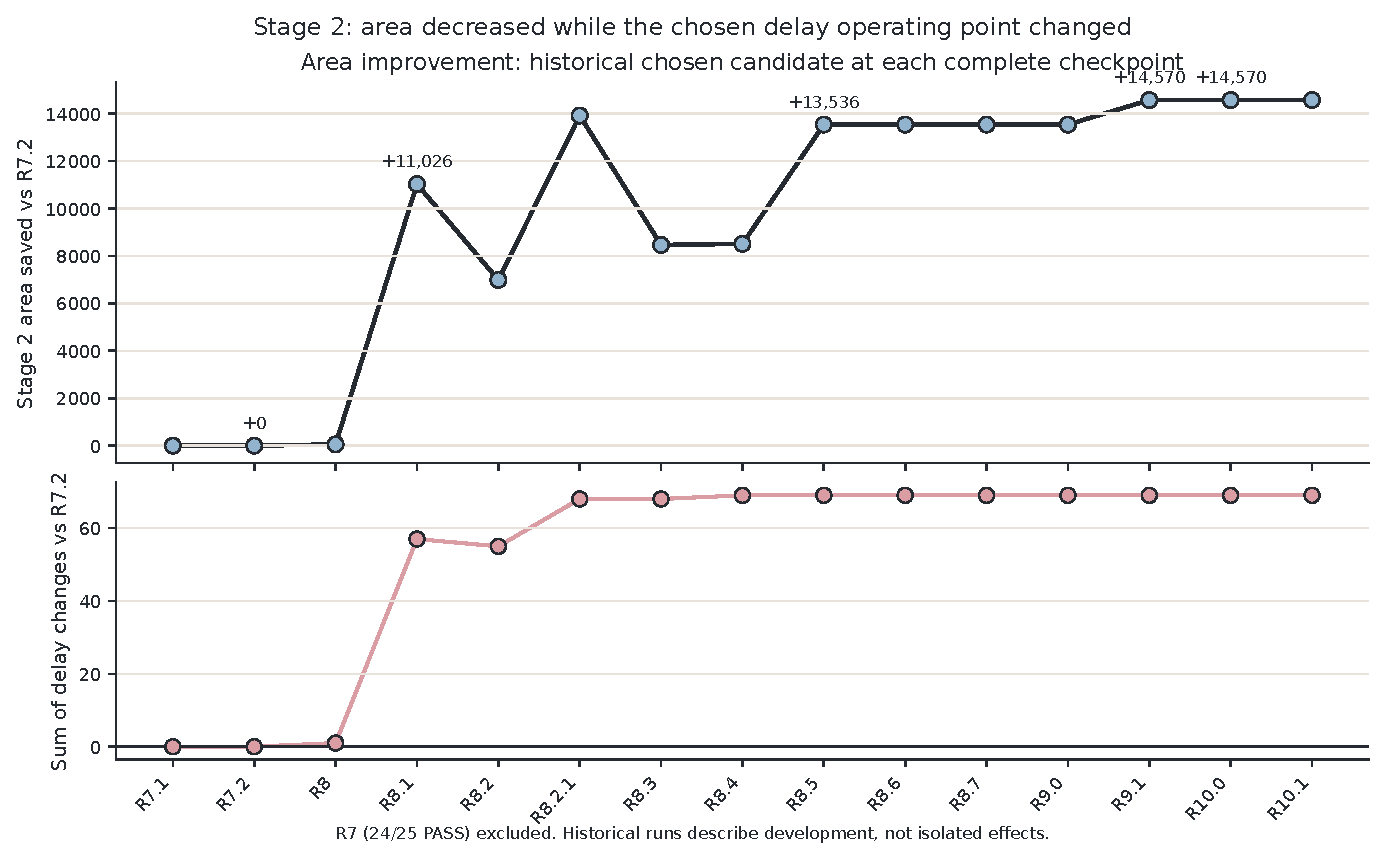
\includegraphics[width=0.98\textwidth]{../figures/14_stage2_area_delay_trajectory.pdf}
\caption{Selected historical Stage 2 area totals expressed as differences from the R7.2 all-passing baseline. Each point is a recorded archived configuration, not a one-factor causal effect. R7's incomplete successful-case total is intentionally excluded; detailed archived pointers are in the verified milestone table.}
\label{fig:long-area}
\end{figure}

Figure \ref{fig:long-aruntime} places each selected archived policy in a two-dimensional \emph{description} of area saved and observed synthesis median. The plot exposes that aggressive search around R8.1 can be costly, and that R8.4's extra search effort did not automatically produce a better point than its neighboring policies. It also shows why a claim that the final frozen algorithm is simply the \emph{fastest} would be inaccurate. Because these medians come from \textbf{different historical campaigns}, we do not draw a randomized causal frontier or quote inter-round speedup factors from these points. Matched R8.6 and R10.0 controls carry the stronger identification claims.

\begin{figure}[htbp]
\centering
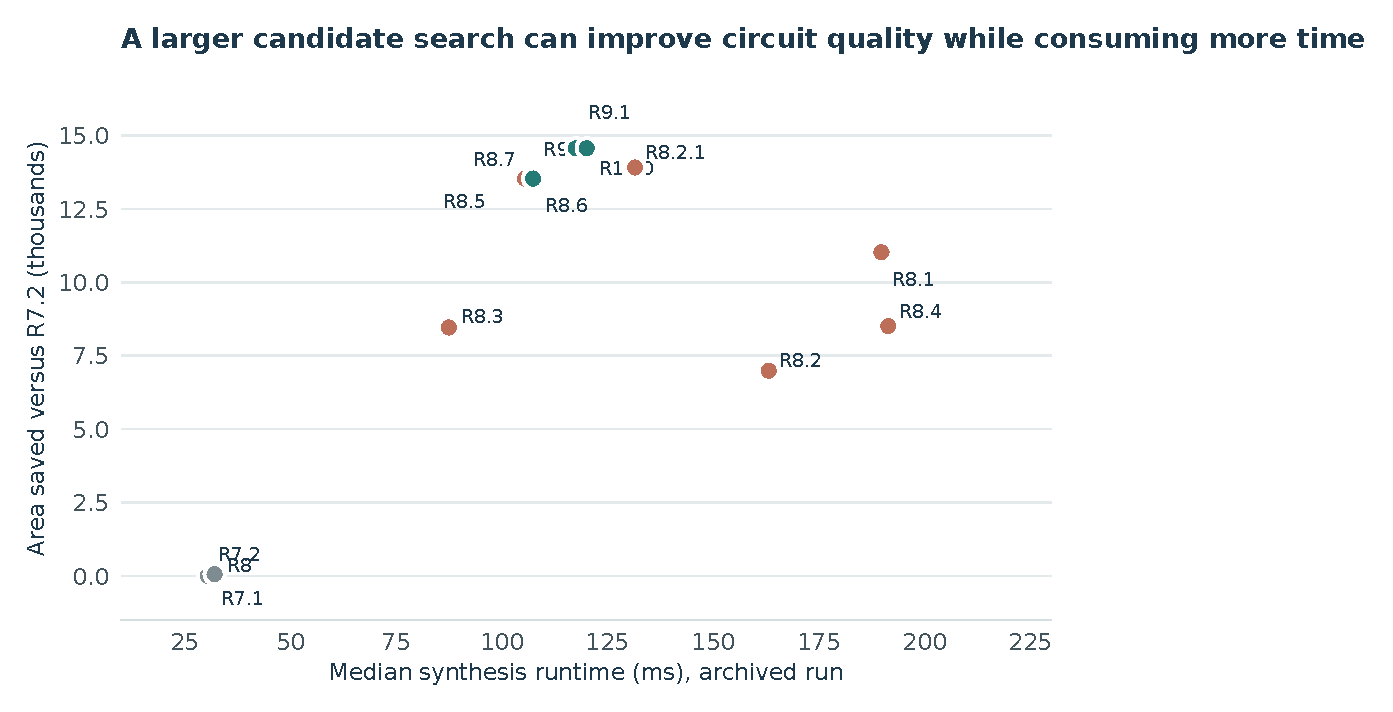
\includegraphics[width=0.93\textwidth]{../figures/02_archival_area_runtime.pdf}
\caption{Area–synthesis-runtime landscape for selected archived Stage 2 runs. The x-axis is program synthesis runtime, not circuit propagation delay. The area baseline is R7.2; scatter locations are descriptive across separately archived experiments and must not be interpreted as a same-run Pareto frontier.}
\label{fig:long-aruntime}
\end{figure}

\subsection{A case-by-round matrix: persistence, reversals and nearly invisible deltas}\label{a-case-by-round-matrix-persistence-reversals-and-nearly-invisible-deltas}

Figure \ref{fig:long-matrix} resolves a question the aggregate trajectory cannot answer: \textbf{are the same functions consistently changing, or does each new strategy discover a different set of opportunities?} Each row takes one designated historical Stage 2 run for a named policy; each column is one released Stage 2 case, all identified by the same bank/case designation. Each cell shows the \textbf{percentage reduction of that case's area relative to its own R7.2 area}, rather than raw gates or a total across differently sized circuits. This normalization makes a 0.5\% change on a small graph perceptible alongside a 36\% change on a structurally different graph. Gray means no reported change.

\begin{figure}[htbp]
\centering
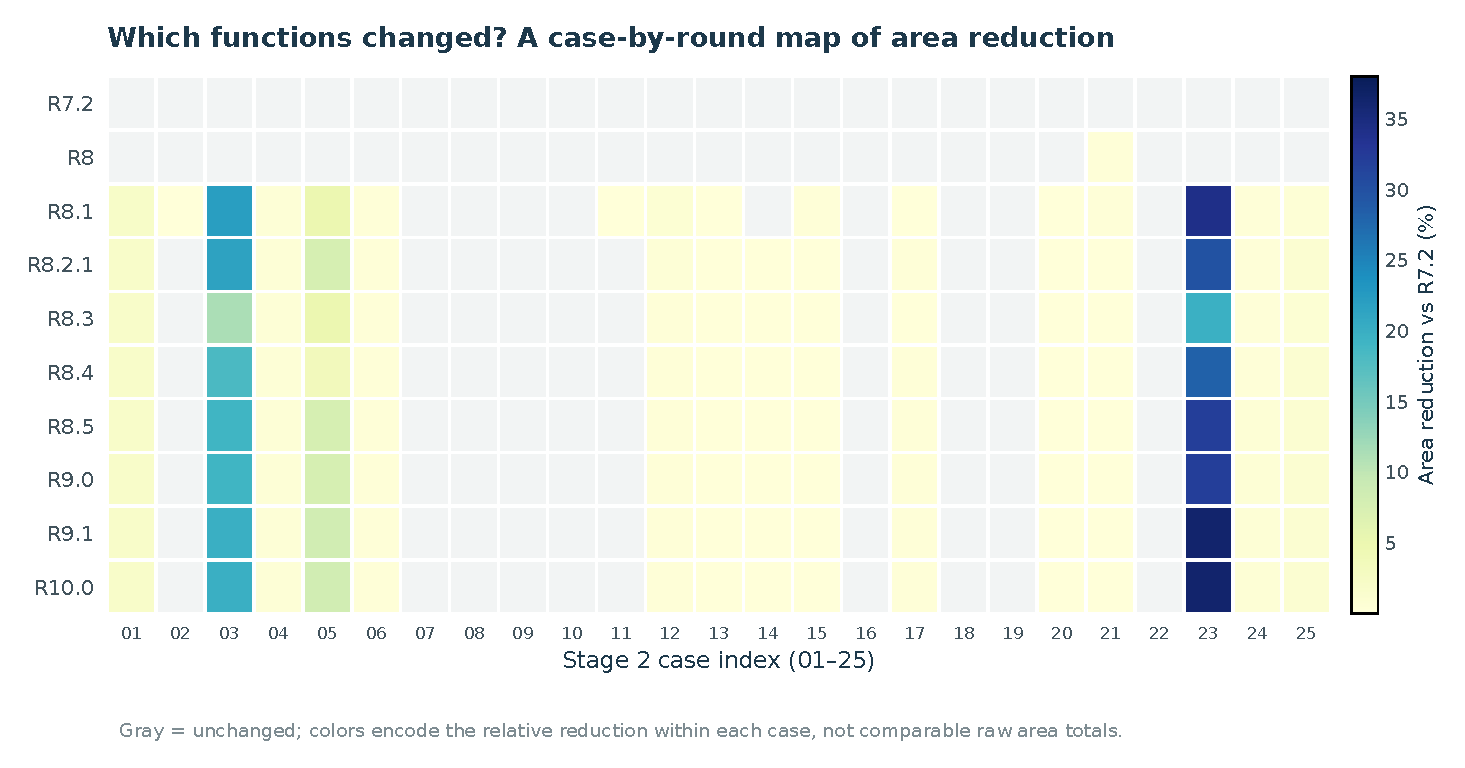
\includegraphics[width=0.99\textwidth]{../figures/03_case_round_area_matrix.pdf}
\caption{Selected Stage 2 historical policies against the frozen R7.2 case-level area baseline; 25 cases per row. Color encodes relative area reduction within an instance. The source table \texttt{casewise\_milestone\_relative\_area.csv} includes full-precision numbers. No causal attribution is made to any one component between two archived rows.}
\label{fig:long-matrix}
\end{figure}

The matrix produces several concrete, checked observations:

\begin{itemize}
\tightlist
\item
  \textbf{Persistence and nonuniversality:} R8.1 changes 17/25 case areas relative to R7.2; R10.0 changes 15/25. In the selected R10.0 Stage 2 benchmark, \textbf{10 cases are unchanged}. This is a statement about the archived 25 inputs, not all Boolean functions.
\item
  \textbf{Nonmonotonic within-case path:} Stage 2 / 003 records approximately \textbf{-21.99\%} at R8.1, relaxes to \textbf{-11.34\%} at R8.3, and settles at \textbf{-19.86\%} at R10.0 relative to R7.2. The historical development does not preserve every early individual win when the runtime and selection policy change.
\item
  \textbf{Long-term concentrated advantage:} Stage 2 / 023 reaches \textbf{-36.24\%} at R10.0, while Stage 2 / 024 reaches only about \textbf{-0.535\%}. The two are both improvements, yet they differ by orders of magnitude in percentage scale. This makes a one-number mean misleading about a typical case.
\item
  \textbf{Small effects are real but must be contextualized:} the R10.0 Stage 2 distribution has a \textbf{median relative area change of approximately -0.052\%} versus R7.2, even though the summed area decreases by 14,570. Five cases improve by at least 1\%, but only two improve by at least 10\%. The total is responding chiefly to a concentrated tail of improvements.
\end{itemize}

These descriptions are \emph{within the same case bank} and hence do not confuse unequal input sets. Still, successive rows are generally \textbf{not matched randomized one-factor treatments}: source code and eligibility policies changed. The matrix reveals \emph{where and when} phenomena occurred; explanations of \emph{which internal cut caused them} require fixed-input DAG traces, not a heatmap.

\subsection{A protocol for using plots as evidence, not illustrations}\label{a-protocol-for-using-plots-as-evidence-not-illustrations}

For each figure in this record, the data extraction script must expose the exact run or report hash, the denominator of cases, and whether an area figure includes only passing cases. Three common mistakes are specifically forbidden: (i) plotting R7's 24-case passing-area sum as though it were a 25-case improvement; (ii) combining a run-1 area with a run-2 runtime to place a fictional point on a tradeoff plot; and (iii) equating a cumulative area win with a majority of case-level wins. The visual form is chosen for the question: a case-by-round matrix for persistence, a sparse lollipop for small localized final changes, a factorial dot plot for controlled knobs, and a sorted contribution plot for distributional asymmetry. None of these establishes a population-level theorem by itself.

The larger arc is now explicit. Stage 1 establishes a correct mapping and efficient candidate engine. R7 makes the process valid under the evaluator's resource envelope. R8 introduces richer function-level cut replacement and exposes the costs of searching it. R8.3--R8.6 distinguish \emph{where} limited work is spent from nominal elapsed allowance. R9.0 protects short-budget execution. R9.1--R10.1 ask whether a narrowly admitted extra SOP pass justifies its time and whether that win survives smaller search caps. This is a \textbf{development explanation supported by distinct experiments}, not a statement that every consecutive version differs by exactly one factor.

\subsection{Multiscale reading of the late research line}
The preceding historical trajectory answers when the candidate-policy regime changed; it cannot resolve a one-thousand-unit gain when the axis spans more than fifteen thousand units. Figure~\ref{fig:late_zoom} therefore uses a separate narrow vertical range. On the Stage 2 bank, the selected checkpoints R8.5 through R9.0 all report area 494,999, while R9.1, R10.0 and the unchanged R10.1 control report 493,965. This is the exact \emph{1,034-unit Stage 2-bank difference}, not the \emph{1,587-unit two-bank difference} of the R9.0--R10.0 paired comparison. The distinction prevents accidental mixing of two aggregation units. These selected archival checkpoints are a development trajectory, not an isolated experiment proving the causal effect of one code edit.
\begin{figure}[htbp]\centering
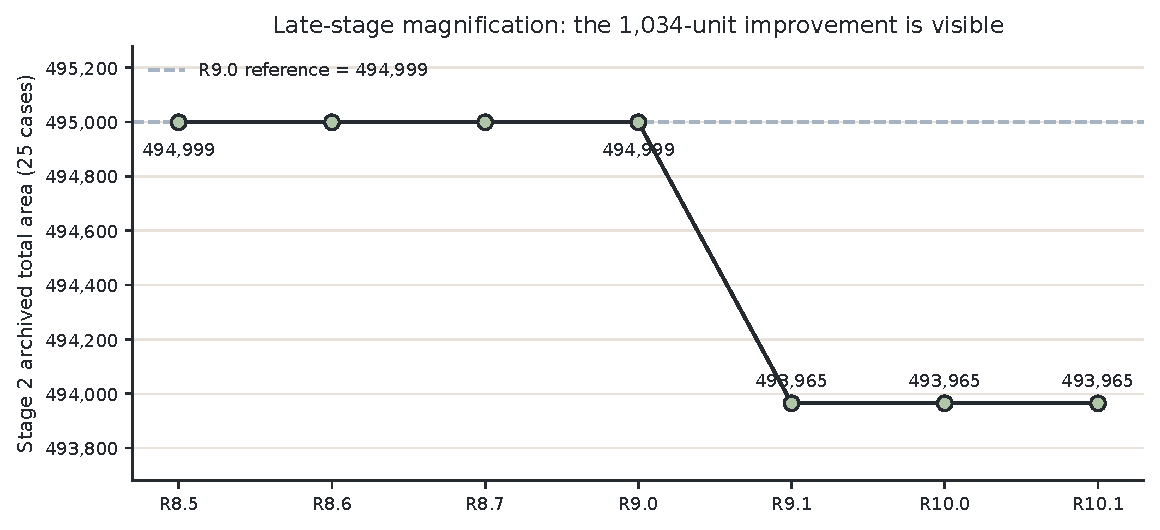
\includegraphics[width=.97\textwidth]{../figures/15_stage2_late_zoom.pdf}
\caption{Late-stage Stage 2 area shown at the resolution needed to see a 1,034-unit change on a roughly 495,000-unit baseline. All points use a complete 25-case checkpoint; cross-version runtime is not inferred from this diagram.}
\label{fig:late_zoom}\end{figure}

\subsection{All 111 named configurations: retain breadth without losing precision}
The experimental inventory contains \textbf{111 distinct (round, variant) names}; \textbf{105} have at least one archived 25-case PASS-and-target-met record, but this does not mean that every repeat of those variants succeeded. The full configuration-by-source listing, including 25-case qualification, observed failures, complete-run minimum/maximum, original report digest, delay, and synthesis runtime, remains in \texttt{data/stage2\_all\_variant\_index.csv}. Rather than presenting eight low-resolution pages of nearly overlapping points, Figure~\ref{fig:variant_spread} asks a more interpretable question: \emph{how much did the alternatives within each Round actually differ?}

The horizontal length is \(\max_v A_v-\min_v A_v\) over qualified archived variants in the same named Round. A symmetric-logarithmic horizontal axis (linear near zero) permits exact zero differences, tens of units, and thousands of units to coexist without making all small differences invisible. The chart thus distinguishes the negligible R7/R7.1/R7.2 variations from broad R8.1--R8.4 exploration, and the more restricted policy changes in R9--R10. It is a \emph{within-Round diversity diagnostic}, not an effect size, confidence interval, or guarantee that the extrema were measured under an interleaved same-executable comparison.
\begin{figure}[htbp]\centering
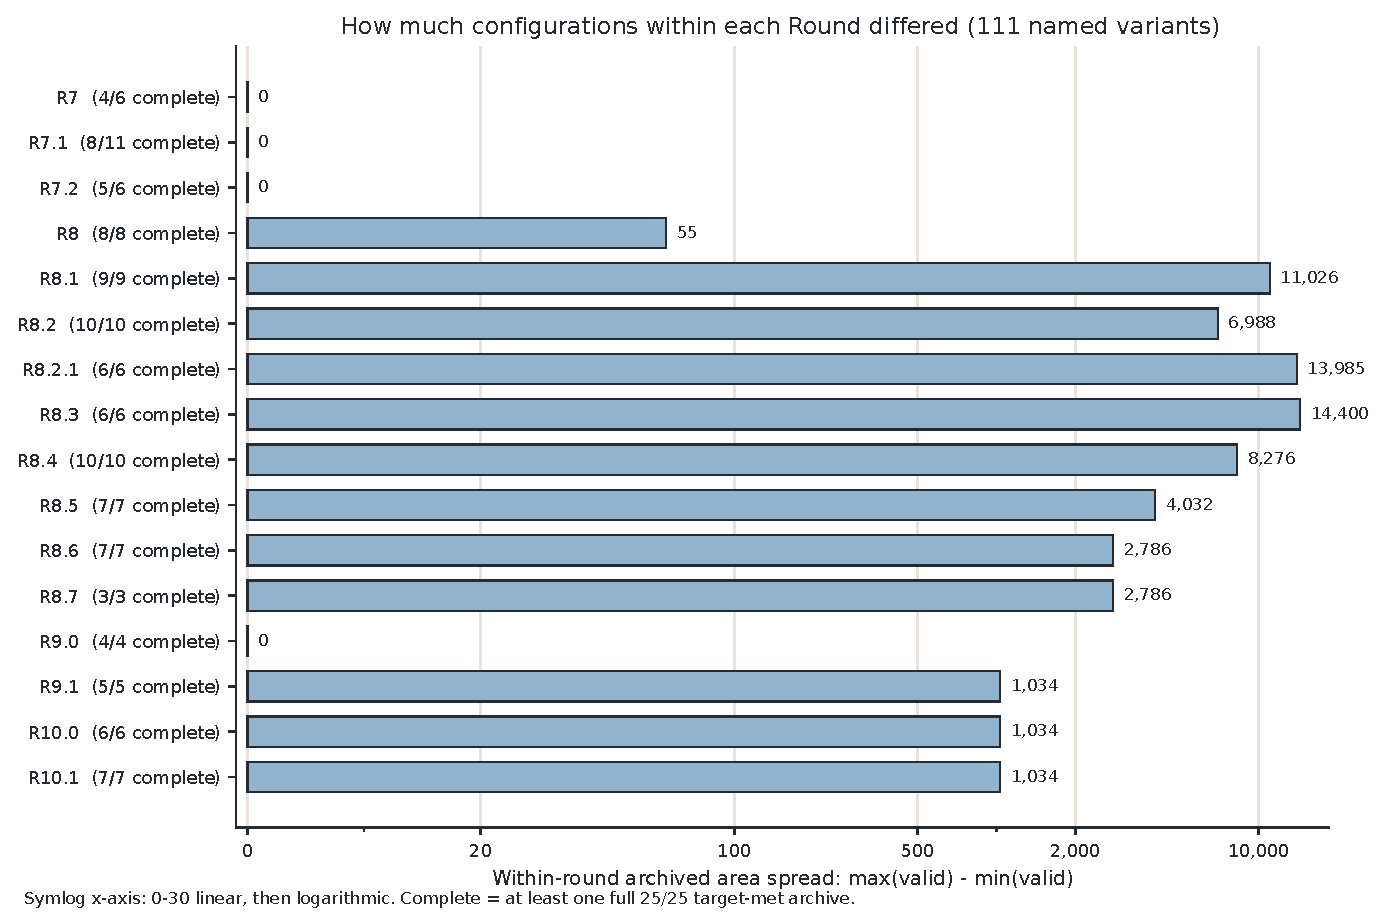
\includegraphics[width=.98\textwidth]{../figures/16_all_variant_spread.pdf}
\caption{Within-Round archived range over complete Stage 2 bank observations, accompanied by qualified/total configuration counts. The horizontal scale uses a linear region near zero and logarithmic growth thereafter; exact original data and evidence paths are preserved in CSV.}
\label{fig:variant_spread}\end{figure}

\subsection{The final policy must be assessed by matched comparison}
The narrow question of whether fewer cut roots or a smaller last-pass budget are preferable \emph{can} be tested on genuinely paired observations. Figure~\ref{fig:archive-finalpolicy} uses 100 matched observations for each R10.1 policy (50 released cases, two repeats). Disabling the final pass yields median runtime ratio \(0.942\) but costs 1,587 weighted area units per 50-case equivalent; caps of 40 and 80 cost 1,008 and 602 units, respectively, while showing only modest median time reductions. A 45-ms allowance costs 241 units and does not improve the observed median runtime (ratio 1.009). Therefore the retained R10.0 policy is a supported \emph{measured operating point}, not a universal optimality theorem or simply the most recent source file.
\begin{figure}[htbp]\centering
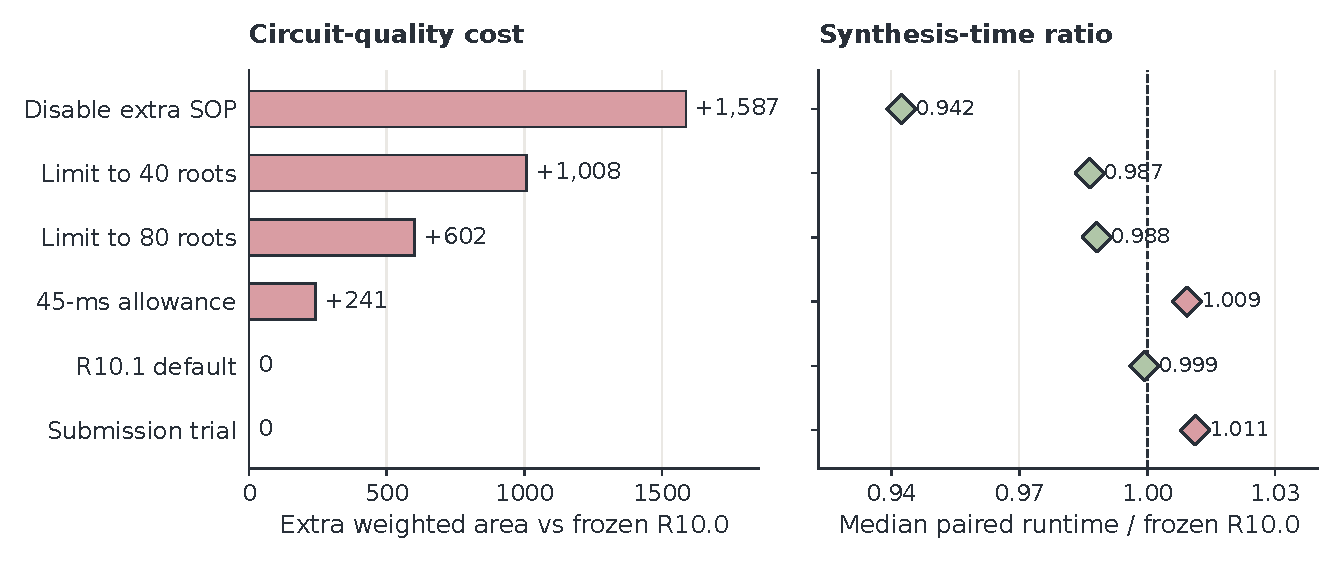
\includegraphics[width=.98\textwidth]{../figures/12_r101_native_pareto.pdf}
\caption{Paired area penalty and synthesis-time ratio relative to frozen R10.0. Positive area penalty is worse; runtime ratios below one are faster. The measurements are converted from 100 paired observations to a 50-case-equivalent area figure.}
\label{fig:archive-finalpolicy}\end{figure}


\section{\texorpdfstring{22. What the development path has \emph{actually} established}{22. What the development path has actually established}}\label{what-the-development-path-has-actually-established}

The trial history is best remembered as an ordered set of \textbf{resolved design questions}, not as a monotone chart of area totals:

\begin{longtable}[]{@{}
  >{\raggedright\arraybackslash}p{(\columnwidth - 6\tabcolsep) * \real{0.2500}}
  >{\raggedright\arraybackslash}p{(\columnwidth - 6\tabcolsep) * \real{0.2500}}
  >{\raggedright\arraybackslash}p{(\columnwidth - 6\tabcolsep) * \real{0.2500}}
  >{\raggedright\arraybackslash}p{(\columnwidth - 6\tabcolsep) * \real{0.2500}}@{}}
\toprule\noalign{}
\begin{minipage}[b]{\linewidth}\raggedright
Phase
\end{minipage} & \begin{minipage}[b]{\linewidth}\raggedright
Initial unanswered question
\end{minipage} & \begin{minipage}[b]{\linewidth}\raggedright
Verified evidence / resolution
\end{minipage} & \begin{minipage}[b]{\linewidth}\raggedright
Explicit limit
\end{minipage} \\
\midrule\noalign{}
\endhead
\bottomrule\noalign{}
\endlastfoot
Stage 1 R1--R3 & Can an exact truth-table circuit satisfy a priced timing target? & Shannon/ROBDD correctness, portfolio mappings and required-time recovery bring released-case target success to 25/25. & Combined improvements not all individually causal. \\
Stage 1 R4--R5.1 & Can near-final area quality be retained at lower synthesis cost? & Selected caching and typed DAG refactors preserve released-case area 529,014; paired runtime falls. & Elapsed-gated future candidates may still vary. \\
Stage 1 R6--Stage 2 R8.1 & Does the mapped DAG contain savings outside original BDD decomposition? & Small-cut semantic resynthesis and direct area/delay controls find additional valid circuits. & Local truth equivalence alone says nothing about whole-DAG area. \\
R7--R7.2 & Can extra search jeopardize validity under a short cap? & Stage 2 / 016 FAIL and guard recovery; shortlist improves an overly conservative quality loss. & A cutoff check is not preemptive worst-case execution-time proof. \\
R8.1--R8.2 & Do area, delay and runtime agree on a best rewrite? & Area-first and strict-delay policies choose different network qualities. & No official scalar score inferred. \\
R8.3--R8.6 & Is effective search work about elapsed wall time or which roots get visited? & Explicit quotas, priorities and factorial contrasts isolate the area benefit of extra SOP roots (2,844) rather than extra nominal time on the released batch. & Not a general theorem about all instance families. \\
R8.7--R9.0 & Are the gains safe to deploy on different structures and constrained runtime? & Generated-function negative result and short-cap stress motivate exact streaming bypass and runtime-first fallback. & A few structured stress fixtures do not bound hidden-case resource use. \\
R9.1--R10.0 & Is a new function library better than an ordinary additional pass? & Library wins more cases but saves less total area; repeat SOP saves 1,587 on eight published cases; R10 default preserves fallback and verifies strict full-DAG improvement. & 0.155\% is an aggregate comparison; typical instance unchanged. \\
R10.1 & Can the final pass be made cheaper without losing its important wins? & Caps 40/80 and 45-ms allowance lose area benefits; no robust runtime-dominance offset. & 160 roots is a tested decision, not a proved global optimum. \\
Independent matched comparison & Does the final program improve over the \textbf{actual submitted} Stage 1 program? & Both methods 50/50 valid; S100 saves 124,697/125,308 area units over the two periods. & S100 loses 32/50 cases by area and is not universally Pareto-superior. \\
\end{longtable}

Three cross-cutting lessons now have an experimentally grounded status:

\textbf{(i) The optimization unit is a whole, priced, timed live DAG.} Shannon and mask equality are function-level guarantees. The four-output counterexample proves that a locally shorter expression can increase full-network area. The R8.1 area--delay results demonstrate why each legal candidate must be rescored, not just locally simplified.

\textbf{(ii) Selecting \emph{useful} work matters more than equating a nominal time budget with optimization progress.} R8.4's rank-vs-topology distinction, R8.6's 2×2 intervention and R9.1's frequency-vs-magnitude reversal show that number of visited candidates, number of winning cases, area payoff and runtime are distinct quantities. The final source uses root caps and reserve rules for exactly that reason.

\textbf{(iii) A release is a \emph{policy}, not a one-off best benchmark value.} R10.0 combines an exact base, optional bounded improvements, strict acceptance and a special short-budget semantic bypass. R10.1's negative result is part of why the frozen default is defensible. This is evidence of reasoned engineering selection rather than a claim of global Boolean minimization.

\section{Reproducing this record and separating what remains unproved}\label{reproducing-this-record-and-separating-what-remains-unproved}

\subsection{Reconstructing an archival comparison without inventing a run}\label{reconstructing-an-archival-comparison-without-inventing-a-run}

\begin{enumerate}
\def\labelenumi{\arabic{enumi}.}
\tightlist
\item
  Identify a named source snapshot and its compiler/evaluator flags; retain the program's full SHA-256 and the case-bank hashes. The frozen source hashes are recorded at the start of this log and in the reproduction bundle.
\item
  Retrieve the matching feedback ZIP or report payload hash; verify that every listed case row is unique, identify PASS versus \texttt{target\_met}, and \emph{exclude FAIL from successful-only numeric area sums without silently reducing the denominator in comparative claims}.
\item
  To compare two policies, join by \textbf{bank, case, period, report experiment and input checksum}. For a genuine one-factor ablation, verify that \emph{all other policy parameters} and the initial incumbent are held fixed. Historical consecutive rounds alone do not establish an isolated treatment effect.
\item
  Report PASS count, target-met count, total charged Area (on explicitly specified common cases), sum or distribution of circuit Delay and paired Runtime summaries. Never substitute circuit Delay for synthesis-time milliseconds; do not interchange \texttt{time\ -v} peak RSS with the evaluator's RAM flag.
\item
  Only after completing the numeric checks, interpret why the \emph{actual source implementation} and mathematical transformation could produce the observed outcome; distinguish what the code makes possible from what an uninstrumented benchmark actually recorded.
\item
  Preserve negative and non-adopted branches. A zero-gain or timeout result can explain a later architecture decision as strongly as an improvement result.
\end{enumerate}

The audit tools accompanying this document reconstruct the raw late-round feedback (\texttt{verify\_raw.py}), re-evaluate every hash-addressed indexed report (\texttt{reverify\_inventory.py}), and retain the detailed normalized outputs. In particular:

\begin{itemize}
\tightlist
\item
  \textbf{\texttt{ALL\_RUNS\_REVERIFIED.csv}:} 1,706 recomputed index rows from 602 distinct content-hash-verified original evaluator tables; 1,706 matched historical aggregate records.
\item
  \textbf{\texttt{RAW\_FEEDBACK\_VERIFIED.csv}:} 196 directly decoded original late-round feedback CSVs, with 25-case completeness, status/target counts, area/delay sums, and runtime summaries; the earliest rounds instead come through the audited evidence database.
\item
  \textbf{\texttt{RAW\_CONTROLLED\_PAIRS\_VERIFIED.csv}:} within-batch contrasts from the native feedback tables, not a noncausal across-archive runtime ranking.
\item
  \textbf{\texttt{RAW\_ARCHIVE\_SHA256.txt}:} archive-level digests linking the late-round measurements to the supplied ZIP bytes.
\item
  \textbf{\texttt{06\_reproducibility/matched\_batch/*.csv}:} 300 newly run/archived three-method invocations covering both banks and both periods. Their figures and hashes originate in the input reproduction package; these files are copied, not secretly rerun during this particular written audit.
\item
  \textbf{\texttt{06\_reproducibility/fixed\_batch/fixed\_order.csv}:} the 24 fixed-graph pass-order arms plus full per-pass counters, signatures and full-truth-table verification traces; experiment executed before this document was authored.
\item
  \textbf{\texttt{06\_reproducibility/scripts/mechanism\_test.cpp}:} source used for the 768 independent small-cut truth checks and the four-output area counterexample, independently compiled and run again for this edition.
\end{itemize}

\subsection{Unproved claims and the exact missing instruments}\label{unproved-claims-and-the-exact-missing-instruments}

The following are not defects that can be fixed by more confident prose. They require different evidence or a narrowed claim:

\begin{itemize}
\tightlist
\item
  \textbf{No exhaustive optimality result:} even a four-leaf mask is exhaustively \emph{evaluated} as a function, but SOP/Shannon/limited template candidates do not enumerate all minimal shared, timing-constrained gate networks.
\item
  \textbf{No measured causal attribution of the production eight R10.0 gains to specific live-node mechanisms:} exact per-case area savings are verified, but an uninstrumented completed-netlist feedback cannot tell how many private nodes died at each particular accepted cut. Required evidence would include frozen incumbent/checkpoint DAGs and per-cut fanout, liveness and arrival logs on a small selected sample. The four-output example demonstrates the mechanism's possibility, not why a particular production case improved.
\item
  \textbf{No full formal runtime/memory guarantee for all allowed tables:} runtime limits restrict performance validity, but periodic guards and exact early recognition do not formally cap every loop or allocator path. Benchmark PASS is an observed property of tested runs.
\item
  \textbf{No representative unknown-input guarantee:} 50 released cases and carefully documented generated families test specific distributions; development tuning on them prevents claims of statistical independence for all later parameters.
\item
  \textbf{No inferred official numerical score:} sum-of-Area, home-made ADP and runtime geometric ratios are explanatory diagnostics. The hidden course score is not reverse-engineered.
\item
  \textbf{No isolated global treatment effect for consecutive multi-change rounds:} where an archived version changes search policy, rooting, cache layout and budget together, a before/after delta is not a one-factor causal estimate. R8.6 and the fixed-incumbent order probe are stronger designs for their narrower questions.
\end{itemize}

\textbf{Research status after this log.} The algorithmic implementation can remain frozen. The full method lineage, successes, negative experiments, feasible tradeoffs and source-backed final policy are now reconstructed for subsequent writing. Only a \emph{limited set of mechanism-level claims} would benefit from additional instrumentation; none should be manufactured to make the existing evidence appear more complete. The next formal Stage 2 paper can be written from this trial record, but its outline is intentionally not precommitted here.

\section{Research appendix A: A compact numerical locator for the Stage 2 sequence}\label{appendix-a.-a-compact-numerical-locator-for-the-stage-2-sequence}

The table below is deliberately an \textbf{index}, not the causal argument. It displays one archived Stage 2 bank, first-period configuration per named round, with the original report SHA-256 and exact source path preserved in \texttt{SELECTED\_ROUND\_MILESTONES.csv}. A multi-version change between two adjacent rows \textbf{must not} be called the marginal effect of one optimization: source conditions, caps, candidate choices and sometimes the evaluation campaign changed. The correct \emph{within-batch} controls are the pair tables, the R8.6 factorial and R10.0 off/default tests described above.

\begin{longtable}[]{@{}
  >{\raggedright\arraybackslash}p{(\columnwidth - 12\tabcolsep) * \real{0.1429}}
  >{\raggedright\arraybackslash}p{(\columnwidth - 12\tabcolsep) * \real{0.1429}}
  >{\raggedleft\arraybackslash}p{(\columnwidth - 12\tabcolsep) * \real{0.1429}}
  >{\raggedleft\arraybackslash}p{(\columnwidth - 12\tabcolsep) * \real{0.1429}}
  >{\raggedleft\arraybackslash}p{(\columnwidth - 12\tabcolsep) * \real{0.1429}}
  >{\raggedleft\arraybackslash}p{(\columnwidth - 12\tabcolsep) * \real{0.1429}}
  >{\raggedleft\arraybackslash}p{(\columnwidth - 12\tabcolsep) * \real{0.1429}}@{}}
\toprule\noalign{}
\begin{minipage}[b]{\linewidth}\raggedright
Milestone
\end{minipage} & \begin{minipage}[b]{\linewidth}\raggedright
Selected policy
\end{minipage} & \begin{minipage}[b]{\linewidth}\raggedleft
PASS
\end{minipage} & \begin{minipage}[b]{\linewidth}\raggedleft
Target-met
\end{minipage} & \begin{minipage}[b]{\linewidth}\raggedleft
Area on passing cases
\end{minipage} & \begin{minipage}[b]{\linewidth}\raggedleft
Delay sum on passing cases
\end{minipage} & \begin{minipage}[b]{\linewidth}\raggedleft
Median synth. ms
\end{minipage} \\
\midrule\noalign{}
\endhead
\bottomrule\noalign{}
\endlastfoot
R7 & default & \textbf{24/25} & 24/25 & \textbf{506,754}* & 1,065* & 33.463* \\
R7.1 & guard & 25/25 & 25/25 & 508,535 & 1,101 & 31.268 \\
R7.2 & shortlist & 25/25 & 25/25 & 508,535 & 1,101 & 30.489 \\
R8 & iterate & 25/25 & 25/25 & 508,480 & 1,102 & 32.131 \\
R8.1 & reverse & 25/25 & 25/25 & 497,509 & 1,158 & 189.880 \\
R8.2 & dual-area & 25/25 & 25/25 & 501,547 & 1,156 & 163.231 \\
R8.2.1 & dual-area & 25/25 & 25/25 & 494,618 & 1,169 & 131.585 \\
R8.3 & stable-dual & 25/25 & 25/25 & 500,072 & 1,169 & 87.518 \\
R8.4 & Top-Q dense & 25/25 & 25/25 & 500,027 & 1,170 & 191.486 \\
R8.5 & budget-reclaim & 25/25 & 25/25 & 494,999 & 1,170 & 104.917 \\
R8.6 & extra-SOP roots & 25/25 & 25/25 & 494,999 & 1,170 & 107.818 \\
R8.7 & extra-SOP roots & 25/25 & 25/25 & 494,999 & 1,170 & 105.535 \\
R9.0 & default no flags & 25/25 & 25/25 & 494,999 & 1,170 & 107.471 \\
R9.1 & repeat SOP & 25/25 & 25/25 & 493,965 & 1,170 & 117.559 \\
R10.0 & default frozen & 25/25 & 25/25 & 493,965 & 1,170 & 120.158 \\
R10.1 & unchanged default & 25/25 & 25/25 & 493,965 & 1,170 & 112.909 \\
\end{longtable}

* \textbf{R7's reported Area, Delay and successful-run median exclude its failed case 016}; they are incomplete metrics and must \emph{not} be treated as a superior 25-case result. R8.1's \texttt{reverse} policy is an area-oriented branch with greater observed delay, \textbf{not} a release decision. R10.1's displayed \texttt{default} is the unchanged control, not a successful new improvement. The Stage 1 bank for these same archived checkpoints, plus original paths, is recorded separately in the paired 32-row CSV.

\newpage

\section{Research appendix B: Source and experiment map: where each technical claim can be checked}\label{appendix-b.-source-and-experiment-map-where-each-technical-claim-can-be-checked}

This map names the archived implementation or original evidence relevant to each research transition, rather than treating a prose statement as proof of code behavior. Root paths below refer to the unpacked user's original \texttt{Stage2\_Final\_Evidence} and \texttt{UFUG2106\_Stage2\_Research\_and\_Reproduction} material.

\begin{longtable}[]{@{}
  >{\raggedright\arraybackslash}p{(\columnwidth - 4\tabcolsep) * \real{0.3333}}
  >{\raggedright\arraybackslash}p{(\columnwidth - 4\tabcolsep) * \real{0.3333}}
  >{\raggedright\arraybackslash}p{(\columnwidth - 4\tabcolsep) * \real{0.3333}}@{}}
\toprule\noalign{}
\begin{minipage}[b]{\linewidth}\raggedright
Technical question
\end{minipage} & \begin{minipage}[b]{\linewidth}\raggedright
Primary implementation / verification source
\end{minipage} & \begin{minipage}[b]{\linewidth}\raggedright
Experimental evidence
\end{minipage} \\
\midrule\noalign{}
\endhead
\bottomrule\noalign{}
\endlastfoot
Stage 1 actual submission versus independent research & Z1 submitted \texttt{src/synth.cpp}; J51 frozen \texttt{src/synth\_round51.cpp} and its headers; 21-page Stage 1 Research Trial Log & Stage 1 frozen development feedback and the two-bank matched batch. \\
R7--R7.2 runtime guards and fallback quality & \texttt{synth.cpp} ancestry; \texttt{UFUG\_R7\_LEGACY\_MERGE} and later schedule/guard branches & R7/R7.1/R7.2 archived official per-case CSV and case 016/020 comparisons. \\
R8 structural patterns and iteration & \texttt{r8\_structural.hpp} & R8 prototype \texttt{off}, \texttt{factor}, \texttt{reuse}, \texttt{strict}, \texttt{all}, \texttt{iterate}; case 021 repeat trace. \\
R8.1 small-cut substitution and typed live-DAG scoring & \texttt{r81\_cut.hpp}, \texttt{r82\_cut.hpp}, \texttt{typed\_netgraph.hpp}, later \texttt{r84\_cut.hpp} & R8.1 SOP/Shannon/strict/reverse controls; local truth-signature correctness test. \\
R8.2--R8.2.1 objective/resource perturbation & \texttt{r82\_cut.hpp}, \texttt{r821\_resource.hpp} & R8.2 dual area/ADP/strict/slack and R8.2.1 restricted-RAM tests. \\
R8.3 work quota and R8.4 Top-Q score & \texttt{r83\_cut.hpp}, \texttt{r84\_cut.hpp} & R8.3 stable/dense/fast, R8.4 ranked/topological/dense tests. \\
R8.5 branch order and R8.6 factorial identification & \texttt{r84\_cut.hpp}, R8.6 dispatch in frozen \texttt{synth.cpp} & R8.5 SOP-first/Shannon-first/budget-reclaim, R8.6 2×2 + reverse control, independently decoded ZIPs. \\
R8.7 distribution and short-limit stress & R8.7 frozen program and generated-case provenance files & \path{experiment/holdout/PROVENANCE.json}, two repeats, tight-budget case logs. \\
R9.0 exact streaming early path & \texttt{r90\_stream.hpp} and early dispatch in frozen \texttt{synth.cpp} & R9.0 official stress fixtures plus published 50-case regressions. \\
R9.1 template versus conventional repeat & \texttt{r91\_library.hpp}, \texttt{r84\_cut.hpp} & Library / repeat-SOP / repeat-Shannon / off controls and casewise results. \\
R10.0 frozen policy and R10.1 no-go & Final \texttt{submission/synth.cpp}, all included headers & R10.0 native \texttt{off}/explicit/default/submission; R10.1 caps and allowance ablations. \\
Cross-stage comparison and pass-order mechanism & \texttt{06\_reproducibility/sources}, \texttt{scripts/fixed\_order.cpp}, \texttt{scripts/mechanism\_test.cpp} & \texttt{matched\_batch/*.csv}, \path{fixed_batch/fixed_order.csv}, exact independent truth-table verification. \\
\end{longtable}

The \textbf{strongest distinction preserved across the log} is epistemic: a source statement explains what a program \emph{can} do, a formal identity explains why a transformation \emph{could} be sound, and a matched experiment establishes what happened \emph{on the measured cases}. None of these three forms of evidence should silently replace another.


